\addchap{\Index{User guide}}

\newcommand{\quicktourFile}{quicktour.avi}

\chapter{Introduction}

\section{Quick ``on the fly'' tour}
\label{sec:quicktour}

In this quicktour you will get a short overview over \icewing{} and
experiment with its GUI. For this you will start a session with a
small video as input and then play a bit with a demo plugin.
With the sources of \icewing{} you got a small video, which you can
use during this tour. It can be found in the docs directory under
the name ``\quicktourFile{}''. Alternatively, you can choose any
other image or video (of a format, that \icewing{} supports).
\index{quicktour.avi}

\paragraph{Compiling the plugin}

During installation of \icewing{} the demo plugin was not compiled
and installed. So let's do that now.
\sS
\shellcom{cd \{wherever your \icewing{}-sources are\} }
\shellcom{cd plugins/demo }
\sE
Now make sure that you have \$\{PREFIX\}/bin in the default-execute
path or, alternatively, change the Makefile in the current
directory. The Makefile needs to find ``icewing-config'', which was
installed in \$\{PREFIX\}/bin. Then simply
\sS
\shellcom{make depend}
\shellcom{make}
\shellcom{make install}
\sE
This compiles the demo plugin and installs it under the name
libdemo.so in the directory \$\{PREFIX\}/lib/iceWing, where \icewing{}
can find it automatically.

\paragraph{The quick tour}

You tell by command line parameters from where \icewing{} will take
its images. There are several kinds of sources: 

\begin{itemize}
\item file-loading from disk (like you do for this session)
\item grabbing from camera\\
  (only available, if \icewing{} was compiled with grabber support)
\item \dacs{} streams\\
  (only available, if \icewing{} was compiled with \dacs{} support)
\end{itemize}

So let's jump in and start \icewing{} with the example plugin ``demo'': 
You launch \icewing{} in the shell-command line with (as one single
line, after changing to the right directory)
\sS
\shellcom{cd \{wherever your \icewing{}-sources are\} }
\shellcom{icewing -sp docs/\quicktourFile{} -l demo}
\sE
After this, \icewing{} opens its main window. At the same time on
the starting console \icewing{} and the plugin write constantly 
their status.

\begin{figure}[h]
  \begin {center}
    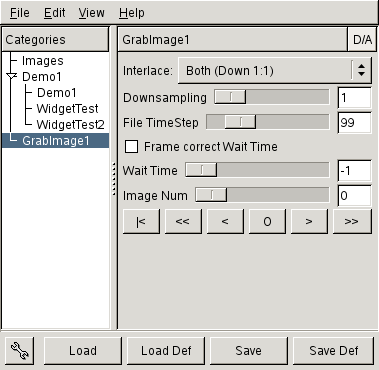
\includegraphics[width=0.6\textwidth]{windowMain}
    \caption{The main window of \icewing{}.}
    \label{fig:windowMain}
  \end{center}
\end{figure}

In figure~\ref{fig:windowMain} you see the \icewing{} main GUI, so lets
explore some things. On the left side you see the ``Categories''
area, which has now ``Images'' and ``GrabImage1'' and some plugin pages.

\paragraph{The category ``\Index{GrabImage1}''}

Click on ``GrabImage1'' to activate this page belonging to the
grabbing plugin, the plugin responsible for accessing images. You
can see several sliders on the right side. If you have during a
session as data source not a video stream but one single image,
``Image Num'' will always be set to 0. None the less \icewing{} has
still the option to (re)acquire that single image on a timely basis:
The slider ``Wait Time'' sets the delay (in ms), after that this
(for video-streams: next) image shall be acquired automatically. If
set to -1, \icewing{} waits until you click manually the read
buttons below. So now set the wait time to 200ms, and you see the
mass of console output greatly reduced.

\paragraph{The plugin pages}

You also launched with the command line parameter ``-l'' one
instance of the plugin ``demo'', which is inside libdemo.so. Every
plugin can generate none or more page-entries on the left
``Category'' side. By selecting the pages you can view plugin status
or change the plugin parameters on the right side. Page ``Demo1''
has some options, that directly affect the plugin. ``Demo1
WidgetTest'' and ``Demo1 WidgetTest2'' not {\em do} anything
useful. But they show you all the available GUI-elements of
\icewing{}, that can also be easily used by your own plugins.

\begin{figure}[ht]
  \begin{center}
    \subfigure[]{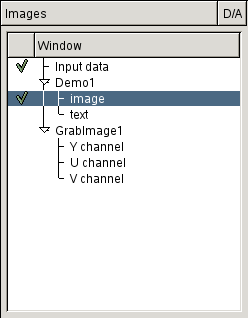
\includegraphics[width=4cm]{windowImages}
      \label{fig:windowImages}}
    \subfigure[]{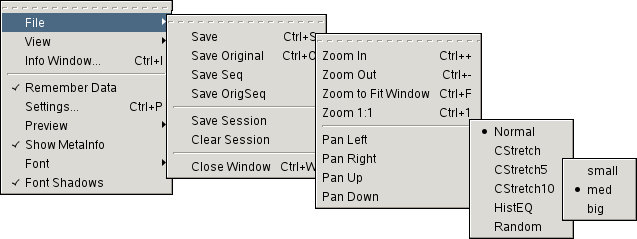
\includegraphics[width=10cm]{menueContextMain}
      \label{fig:menueContextMain}}
  \end{center}
  \caption{(a) The page ``Images''.
    (b) The context menu of window ``Demo1 image'' with all its submenus.}
\end{figure}

\paragraph{How to display plugin results?}

With click on category ``Images'' you see on the page on the right
side several ``Window'' entries coming up (see
figure~\ref{fig:windowImages}). They show you all windows that the
plugins wish to display. Double-click (de)activates the window of
that entry and you can see what the plugins are doing.

You see one window ``Input data'' for the current input image, one
separate window for each YUV channel of the source image and two
windows for the output of the plugin instance ``Demo1''.

Lets now activate the first demo window called
``Demo1.image''. Inside this new window press the right mouse button
and verify that ``Remember Data'' is active (see
figure~\ref{fig:menueContextMain}). This flag makes all coming zoom
commands operate on the currently loaded image data, not only on
{\em new} acquired/grabbed images. If you deselect this option, and
e.g. try to zoom around, the zoom commands will still be remembered
- but the window content will still display (unchanged until next
image reading) the last acquired image without any of the zoom
commands visible. When you set ``Wait Time'' = -1, you see the
``Remember Data'' flag's functionality very clear: When ``Remember
Data'' is inactive, only reloading the image source will refresh the
window content and show your until then done zooms.

\paragraph{Zooming the window content}

Inside the window shift/crtl/alt-keys plus middle mouse button zoom
in/out/reset the image. When you just hold the middle button and
move the mouse around, you can pan inside the image, if you have
zoomed into it. Additionally, you can use the scroll whell and the
shift and ctrl-keys to pan and zoom in the window, or, as a third
option, the ``View'' context menu. If you have problems with the
zooming, look at the section~\ref{sub:panZoom}
``Panning/Zooming the image windows''.

Now play a bit with the ``Remember Data'' flag and ``Wait Time'' and
zooming to work it out.

\paragraph{Manipulating image colors}

In the context menu (right mouse button) you can see the
``Preview-\textgreater{}Random'' option. This tool randomizes the
color assignments. This can be useful to verify the output of a
color separating plugin, because very similar/neighbored colors now
get very distinguishable.

\paragraph{Saving the zoomed part into a separate file}

After you played around a bit, you can safe the frame content into a
file with context menu entry ``File/Save''. The picture will be the
window content and its name be ``Gsnap\_0.ppm''. If you wish a
different name/format, you can change this (and more) by clicking
the wrench icon of the main Window (see figure~\ref{fig:windowMain}) to
get the preferences window. There you can change the image name to
e.g. ``quicktour\_zoomed\_\%d.ppm'' (the \%d is a placeholder for
the image number).

\paragraph{More about this plugin via ``Plugin info''}

From the menu in the main window (figure~\ref{fig:windowMain})
select ``View/Plugin Info''. Here you see how the plugin instance
``Demo1'' is integrated into the \icewing{} system, You see the
sheet and the only two enabled plugins with own instances are
``Demo1'' and ``GrabImage1''. The plugin instance ``GrabImage1''
from the ``grab'' plugin is needed to acquire the image from hard
disk (command line parameter ``-sp''). All other plugins (``record''
etc.) are further inbuilt or installed ones, but they are not
registered into the current session of \icewing{} and thus have no
active instances.

More of this all later in the section~\ref{sub:PluginInfo} ``Plugin
Info''...

%######################
\section{The special plugin ``grab''}

\paragraph {The plugin ``grab''}

is a very basic and thus inbuilt plugin, that allows to acquire
images or video streams from grabber hardware, disk or via \dacs{}
from external processes. This plugin will be used by nearly all
other image processing plugins. But \icewing{} not {\em needs} this
plugin! But then you need your own plugin as ``data-provider'' for
e.g. audio streams or likewise.

\paragraph {Some comments on up-/downsampling}

\icewing{} provides the images via the plugin ``grab'' (or other
data-provider plugins). And the plugin ``grab'' provides two
separate queues of image histories: downsampled and upsampled
(i.e. full/original sized) images. With a downsample factor of 1 the
two queues have the same images, while a factor of 3 makes the
downsampled images consist of every 3rd pixel of the original sized
image. Both queues have a history size - how many images will be
stored for plugin access to older images. Excellent - but what for?

Well, this feature is useful when both reduced and detailed image
size versions are needed for the global task. E.g. a continously
operating plugin ``trajectory tracking'' uses the faster downsampled
images to swiftly keep track of the hand-position. Meanwhile, but
much less frequently, another very time-intensive plugin ``object
detection'' separates an object in that hand. For this job, it may
register for the more detailed queue of upsampled images.

\chapter{The command line interface}

\section {The \Index{command line parameters} in detail}
\label{sec:commandline}

\shellcom{icewing -h}
\sE
gives you the list of command line parameters. Now they will be
explained more detailed, arranged to subject.

\subsubsection {General options}

\begin{description}
\item[@\textless{}file\textgreater{}]
  This allows to store arguments in files. Option ``@'' replaces
  its argument \textless{}file\textgreater{} with the content of
  \textless{}file\textgreater{}. Any lines in
  \textless{}file\textgreater{} starting with '\#' are ignored, the
  remaining lines are treated as further options.

\item[-h \textbar{} --help]
  Besides showing all options and there meaning \icewing{} writes
  the names of all plugin instances, that are created by parameter
  ``-l'' or ``-lg'' and then terminates. You need the precise names
  of the plugin instances if you wish to send options to specific
  plugin instances with option ``-a''.

\item[--version]
  Shows version information and exits the program.

\item[-n \textless{}name\textgreater]
  \label{page:opt_n_name}
  When you use \dacs{}, the launched instances of \icewing{} must be
  somehow addressable. This option specifies the process name of this
  instance of \icewing{} - the default name is ``icewing''. If there
  are several instances of \icewing{} (network wide), you must care:
  Give at least those \icewing{} processes unambiguous names, that
  are used with \dacs{}.

\item[-p \textless{}width\textgreater{}x\textless{}height\textgreater{}]
  Sets the size of preview windows, default: 384x288.

\item[-rc \textless{}config-file\textbar{}config-setting\textgreater{}]
  If the argument to this option contains a '=', the argument is
  interpreted as a gui setting and the referenced gui element is
  modified accordingly. Otherwise, the given config file
  \textless{}config-file\textgreater{} is loaded {\em additionally}
  to the standard file ``\$\{HOME\}/.icewing/values'' (which is read
  first). This option can be given multiple times.

\item[-ses \textless{}session-file\textgreater{}]
  Load the session file session-file {\em instead} of the standard
  file ``\$\{HOME\}/.icewing/session'' and use this file for any
  session related operations.

\item[-time \textless{}cnt\textbar{}plugins\textbar{}all\textgreater{}...]
  ``cnt'' specifies after how many main loop iterations time
  measurements are given out. If ``cnt''\textless{}=0 all time
  measurements are disabled. The default is 50. The other arguments
  allow to automatically create timers for measuring the execution
  time of the process() call for single plugin instances. If ``all''
  is given, all plugin instances are measured. For example

  \shellcom{icewing -time ``5 backpro imgclass''}
  \sE
  outputs time measurements all 5 main loop runs and creates timers
  for the plugin instances backpro and imgclass. This option can be
  given multiple times.

\item[-iconic]
  Start the main \icewing{} window iconified.

\item[-t \textless{}talklevel\textgreater{}]
  \label{page:opt_t_talk}
  \icewing{} outputs debug messages only if their level is below
  \textless{}talklevel\textgreater{}, default: 5, used range of
  levels: 0..4.

\end{description}

\subsubsection {Input options}

\emph{Remember}: All this options, that are related to image input
(-sg, -sp, -sp1, -sd, -prop, -nyuv, -nrgb, -c, -f, -r, -stereo,
-bayer, -crop, -rot, and -oi) are passed to the special plugin
``grab''. If you use another plugin as data-source, that plugin will
have its own input options (passed via ``-a''). Neither ``grab''
knows of the other plugins options, nor does the other plugin see
this input options.

So {\em this} options could also be thought as ``input options for
plugin grab''. You can use multiple instances of the plugin grab and
thus multiple images at the same time. If you want to do that, you
have to pass these options via the \icewing{} option ``-a'' to the
additional grab instances. Thus every instance of grab can get its
very own options. The multiple instances are created by loading the
plugin via the option ``-l'' multiple times.

\begin{description}

\item [-sg \textless{}inputDrv\textgreater{} \textless{}drvOptions\textgreater{}]
  {\em S}ource of {\em G}rabber: If you use a grabber camera for
  your images and you compiled \icewing{} with grabber support, you
  can select with this option how to access your grabber hardware.
  \icewing{} supports several camera systems, and here you select
  which you use.

  \textless{}inputDrv\textgreater{} can be, depending on how you
  compiled \icewing{}, one of PAL\_COMPOSITE, PAL\_S\_VIDEO, V4L2,
  ARAVIS, FIREWIRE, ICUBE, MVIMPACT, UEYE, or UNICAP (or
  abbreviated ``C'', ``S'', ``V'', ``A'', ``F'', ``I'', ``M'',
  ``E'', and ``U''). See section~\ref{sec:para_driver} for more
  details about the different drivers.

  \textless{}drvOptions\textgreater{} is an option string, which
  specifies in more detail how the driver you selected with
  \textless{}inputDrv\textgreater{} should behave. The different
  options of the drivers are described in section~\ref{sec:para_driver}.

  The different drivers provide help for its driver options: If you
  are not sure, which options your selected driver, e.g. ``F'', the
  firewire driver, has, try
  \sS
  \shellcom{icewing -sg F help}
  \sE
  and an overview of the options will be printed to the console.

  If you only give -sg without anything special, the default setting
  is PAL\_S\_VIDEO with no special options. 

\item[-sp \textless{}fileset\textgreater{}]
  {\em S}ource of {\em P}ictures: What you specify as
  \textless{}fileset\textgreater{} will be the picture(s)
  data-source for the plugin ``grab''. Reaching the last picture
  \icewing{} loops, beginning again with the first picture.

  \icewing{} natively supports the \emph{pnm} image
  format and two AVI formats with a RAW codec. Depending on your
  version (or if installed at all) of the gdk-pixbuf library, the
  range of supported image formats is greatly enhanced. Version 0.16
  provides e.g. this formats: \emph{bmp}, \emph{gif}, \emph{ico},
  \emph{jpeg}, \emph{png}, \emph{ras}, \emph{tiff}, and
  \emph{xbm}. \emph{pnm} images are read in bit depths from 8 to 32
  and in special variants float and double images can be read,
  too. \emph{png} images are read in 8 bit and 16 bit depths. All
  other formats are 8 bit only.

  \textless{}fileset\textgreater{} specifies the list of file
  names. It has the following format:\\
  \hspace*{0.9cm}fileset = fileset \textbar{} 'y' \textbar{} 'r'
  \textbar{} 'e' \textbar{} 'E' \textbar{} 'f' \textbar{} 'F' \textbar{} 'file'

  \begin{description} %-sp

  \item [Single Pictures]
    You can simply give single pictures as files
    \sS
    \shellcom{icewing -sp image.ppm image2.gif}

  \item['y', 'r' $\rightarrow$ YUV or RGB]
    The pictures can be stored as color model YUV or RGB (which is
    the default). With a 'y' or 'r' in front of the name you
    can specify the color model of the coming files. So this example
    names one RGB, two YUV and another RGB picture as data source
    sequence:
    \sS
    \shellcom{icewing -sp imageRGB1.ppm y imageYUV1.ppm imageYUV2.ppm r imageRGB2.ppm}

  \item['file' with \%d or any int based printf() conversion specifier]
    As further option you can name a whole series of pictures: with
    e.g. \%d the plugin ``grab'' replaces \%d by integer numbers
    beginning from 0 and tries to open the file. As another example
    ``\%04d'' matches all numbers, starting with 4 leading zeros. As
    soon as \icewing{} cannot match the current number, it moves on
    to the next fileset. E.g.

    \shellcom{icewing -sp image\%03d.ppm picture\%d.ppm}
    \sE
    makes the plugin ``grab'' increasingly scan for (and if found:
    load) files named with ``image000.ppm'', ``image001.ppm''... If
    no further file is found, it scans for pictures named
    ``picture0.ppm'', ``picture1.ppm''...

  \item['file' with at least \%t or \%T, or a combination of \%t, \%T, and \%d]
    \label{page:opt_sp_time}
    An alternative method to specify a series of pictures, one
    example would be '/tmp/image\%T\_\%t.png'. If \%t or \%T is
    inside the file name part of one 'file' to the -sp option,
    \icewing{} scans the complete directory, in the example '/tmp',
    for files matching the file name part with any numbers replacing
    \%d, \%T, and \%t. It loads the found files sorted by the
    numbers replacing \%d, \%T, and \%t in that direction. I.e. the
    coarsest order is given by \%d and the finest by \%t.

    In this case no printf() style format specifiers are allowed, as
    files with any number format are used at the same time.

  \item['e', 'E' $\rightarrow$ Open files/Check file extension]
    \icewing{} must know the number of images you specified on the
    command line. To verify if a file is a movie file and then get
    its frame count, \icewing{} opens every file during
    startup. With an 'E' in front of the file names \icewing{} opens
    only these files which have a known movie extension
    (e.g. '.avi' or '.ogm'). This speeds up the program start. With
    an 'e' in front of the file names you switch back to opening all
    files. The default is to open all files.

  \item['f', 'F' $\rightarrow$ Duplicate/No duplicate frames in movies]
    Movie files store the number of frames to display in one second
    (FPS value) and the to be displayed frames. Normally, if less or
    more frames are stored in the movie at one point in time than
    the number of frames, which had to be available according to the
    FPS value, single frames get duplicated or removed. If 'F' is
    specified, this duplication and removal does not happen.
    In this case, the ``Image Num'' slider in the user interface on
    the ``GrabImage1'' page (see page \pagereftop{page:gui_image_num})
    can only be used for seeking if the read continuous buttons
    ('\textless{}\textless{}' and '\textgreater{}\textgreater{}')
    are not pressed. The default is to comply with the FPS value.

  \end{description} %-sp

\item[-sp1 \textless{}fileset\textgreater{}]
  This is just the same as -sp. But after the last picture is
  reached and every registered plugin has finished its work on that
  picture, the \icewing{} process ends instead of looping back to
  the first picture.

\item[-sd \textless{}stream\textgreater{} [synclev{]}]
  Use a \dacs{} stream as input of images (for plugin ``grab'').

  An external process creates that stream of images somewhere in the
  network. It has published it via \dacs{}, and this \icewing{}
  process can order that stream as input of images.

  The stream can have some synchronize-tokens of several hierarchical
  levels integrated. This SYNC-tokens of increasing level create
  substructures of the incoming data (e.g. letters, words,
  sentences...). You can register the stream at a given
  synclevel. Level 0 means {\em every} single image will be
  delivered to this \icewing{} instance. Higher levels lead to fewer
  images, depending strongly on the SYNC-level philosophy of the
  stream creating process. You need to get this information about
  the stream creating process to choose the appropriate SYNC-level,
  with that you register the \dacs{} stream. If the stream
  delivering process separates the images with SYNC-level 2 and you
  order this stream at this level, you will get always the latest
  image. Any older images get dropped off the stream, as soon as the
  new image arrives the stream. So with this strategy \icewing{}
  gets always up to date images - simply by ordering at the
  appropriate level.

  {\em Caution:} SYNC-level of 0 is {\em special} and means, that
  this instance of \icewing{} gets {\em every} single image, that is
  put into the stream (no loss of any image). You may need this,
  e.g. because plugins sometimes need access to older, but still
  unreceived images. But the \dacs{} process must store all of the
  undelivered images. If \icewing{} consumes the images at a slower
  rate than the images are put into the stream (in average), this
  will definitely lead sooner or later to a {\em huge} size of the
  \dacs{} process -- and finally (when the storage limit is
  exceeded) the process gets killed by the system.

  If you wish write your own image-creation process to send images
  to \icewing{} via \dacs{}: There is already the SFB-360 internal
  data type ``struct Bild\_t'' (which is declared in the file
  ``sfb.h''). It encodes the image, and you must use it as the type
  to be passed to \dacs{}. Then \icewing{} can receive images from
  your own process.

  For further details about \dacs{} see the dissertation of Nils
  Jungclaus \cite{Jungclaus1998-IVS}.

\item[-prop]
  Normally, when you use a grabber, see option ``-sg'', and the
  grabber supports changing properties on the fly, a GUI in form of
  an own page in the categories list is created to change these
  properties interactively. When you use ``-prop'' this page is not
  created.

\item[-stereo]
  Expect gray images containing interlaced \Index{stereo images} as
  input and decompose them by putting them one after the other. This
  option is similar to the ``stereo=deinter'' option of the V4L2
  driver (see section~\ref{sub:para_v4l2} for more details).

\item[-bayer [method{]} [pattern{]}]
  Expect a gray image with an embedded \Index{bayer pattern} as the
  input image. Use the specified method and the specified bayer
  pattern to decompose it. If no method or pattern is specified,
  downsampling and RGGB are used. The supported methods are:
  \begin{description}
  \item[down] Downsampling of the input image by a factor of 2.
  \item[neighbor] Nearest neighbor interpolation.
  \item[bilinear] Bilinear interpolation.
  \item[hue] Smooth hue transition interpolation.
  \item[edge] Edge sensing interpolation.
  \item[ahd] Adaptive homogeneity-directed interpolation.
  \end{description}
  Supported bayer patterns are: RGGB \textbar{} BGGR \textbar{} GRBG
  \textbar{} GBRG.

  This option is similar to the ``bayer'' and ``pattern'' options of
  the V4L2 driver (see section~\ref{sub:para_v4l2} for more
  details).

\item[-crop x y width height]
  Crop a rectangle starting at position (x,y) of size width x height
  from the input image. If width or height are smaller than zero or
  zero, the values are measured from the right or bottom
  side. E.g. ``-crop 5 10 -5 -10'' would crop a border of 5 pixel
  from the left and right sides and a border of 10 pixels from the
  top and bottom sides of the input image.

\item[-rot \{0 \textbar{} 90 \textbar{} 180 \textbar{} 270\}]
  Rotate the input image by $0^\circ$, $90^\circ$, $180^\circ$, or
  $270^\circ$. The default is $0^\circ$.

\item[-nyuv \textless{}name\textgreater{}] \icewing{} provides its
  input images for other plugins under a special name, normally
  ``image'' for YUV images. With this option you can change this
  identifier to \textless{}name\textgreater{}. See the
  paragraphs~\ref{para:observingData} and \ref{para:pluginSupport}
  for alternatives plugins should normally use.

\item[-nrgb \textless{}name\textgreater{}] \icewing{} provides its
  input images for other plugins under a special name, normally
  ``imageRGB'' for RGB images. With this option you can change this
  identifier to \textless{}name\textgreater{}. See the
  paragraphs~\ref{para:observingData} and \ref{para:pluginSupport}
  for alternatives plugins should normally use.

\end{description}

\subsubsection {Options for up-/downsampling behavior}
\index{Downsampling}

\begin{description}
\item[ -c \textless{}cnt\textgreater{}]
  \icewing{} internally manages a queue of downsampled images. With
  this option you can specify the length of this queue.

  Default value is 2.

\item[ -f [cnt{]}]
  If you do not specify this option, \icewing{} has only the
  downsampled queue of images. With ``-f'' \icewing{} activates the
  {\em F}ull sized (i.e. the upsampled) queue of images.

  The optional [cnt] sets the queue size, the default is 1.

\item[-r \textless{}factor\textgreater{}]
  {\em R}emember downsample factor of input images.

  If you use already downsampled images as input, unfortunately
  \icewing{} does not know this without further
  notifying. \textless{}factor\textgreater{} tells the interested
  plugins, what factor the source images got downsampled.

  Remember: With downsampled image sources, plugin grab will {\em
    additionally} downsample the input into the downsample queue. So
  when the input images already have downsample factor of 2, and the
  current \icewing{} instance has downsample factor of 3, the images
  in the downsample queue will have a {\em true} downsample factor
  of 6 (compared to the original image), while the images inside
  the upsampled queue have downsample factor of 2. The only way to
  solve this and e.g. simulate the original size of the image is to
  use this option ``-r'': You tell \icewing{}, what downsample
  factor the input images already have. And the plugins can (but not
  need to) make use of this additional information.

  And also remember: Even the commando ``Save Original'' saves the
  original (=unrendered) image, but {\em including} the given
  downsample factor (set in figure~\ref{fig:windowMain} page
  ``other'' or in paragraph Downsampling~\ref{para:downsampling}).

\end{description}

\subsubsection {Output/remote control options}

The ``-o'' options have several different purposes regarding the
communication to other programs and with the sub options
you specify, what to output and what interfaces to enable.

\begin{description}

\item[-of]
  \label{page:opt_of}
  With option ``-of'', this instance of \icewing{} can be fully
  remote controlled via \dacs{} including nearly every single
  GUI-widget element.

  This uses the capability of \icewing{} to save and load all its
  current status into the config file (while session file stores the
  window properties). Remote control via \dacs{} works quite
  similar: With this option ``-of'' \icewing{} publishes \dacs{}
  wide the functions
  void \textless{}icewing\textgreater{}\_control(char[]) and
  char[] \textless{}icewing\textgreater{}\_getSettings(void).
  \textless{}icewing\textgreater{} is the name of this instance of
  \icewing{} (that you specified with option ``-n''). The ``char[]''
  means, that you send a normal C-string as parameter to the
  \_control() function. The content of that string can be any lines
  of the \icewing{} configuration file and \icewing{} accepts the
  new settings. Similar, the \_getSettings() function returns a
  string with the current settings of all widgets in the format of
  the configuration file. See also the icewing-control program from
  the utils directory for a utility, that allows to send such
  strings to a running \icewing{} instance. See
  section~\ref{sec:icewing-control} for more details about this
  utility.

  Additionally this option publishes to \dacs{} the function
  struct Bild\_t \textless{}icewing\textgreater{}\_getImg(imgspec).
  With this function, external processes can receive an image from
  this instance of \icewing{} via \dacs{}. The images are send
  encoded in the SFB-360 ``struct Bild\_t'' data type. There are
  further options, to allow the external process to select precisely
  which image it receives, and in which downsample format. 

  The format of ``imgspec'':
\begin{verbatim}
    ['PLUG' <plugnum>] ('NUM' <imgnum>|'TIME' <sec> <usec>|
    'FTIME' <sec> <usec>) down
\end{verbatim}

  \begin{description}

  \item[PLUG]
    If multiple instances of the plugin grab are running, multiple
    images are available at the same time. With PLUG you can select
    the image from the instance
    \textless{}plugnum\textgreater{}. The default is 1, i.e. the
    image from the first grab instance.

  \item[NUM]
    Every single image in \icewing{} has a continuous number,
    starting with 0. \icewing{} returns the image with the number
    \textless{}imgnum\textgreater{}. If
    \textless{}imgnum\textgreater{}\textless{}0, return a full size
    image, see option ``-f''. If \textless{}imgnum\textgreater{}=0,
    return the current full size image.

    So the sign determines, from which queue \icewing{} takes the
    image from: the upsampled or the downsampled queue (See also
    options ``-c'' and ``-f'').

    If the upsampled queue is not existing, you will always get the
    downsampled version of the image.

  \item[TIME]
    \icewing{} returns that image with a grabbing time most similar
    to (\textless{}sec\textgreater{}
    \textless{}usec\textgreater{}). The image is taken from the
    downsampled queue.

    If TIME is in the future, the nearest image is taken - and that
    will always be the most recent image.

  \item[FTIME]
    \icewing{} returns a full size image with a grabbing time most
    similar to (\textless{}sec\textgreater{}
    \textless{}usec\textgreater{}).

    Again, if the upsampled queue is not existing, you will always
    get the downsampled version of the image.

  \item[\textless{}down\textgreater{}]
    \icewing{} will downsample the returned image by factor
    \textless{}down\textgreater{}. This factor is applied {\em
    additionally} to the \icewing{} downsample factor (adjustable in
    page ``GrabImage1'', see figure~\ref{fig:windowMain})!

    As example: \icewing{} has set a downsample factor of 2 and this
    option \textless{}down\textgreater{} is e.g. set to 3. Now the
    image will be delivered to \dacs{} with a true downsample factor
    of 6 (well, with FTIME it is 3).

 \end{description}

\item[-oi [interval{]}]
  Output images on \dacs{} stream
  \textless{}icewing\textgreater{}\_images and provide a function
  void \textless{}icewing\textgreater{}\_setCrop(``x1 y1 x2 y2'') to
  crop the streamed images. \textless{}icewing\textgreater{} stands
  for the \dacs{} name of this \icewing{} process (see option
  ``-n''). With the optional [interval] \icewing{} will send
  only every nth image to the stream. If the upsampled queue exists,
  you will get an upsampled image, otherwise a downsampled
  image. The images are sent in the ``struct Bild\_t'' format.

  With the function \textless{}icewing\textgreater{}\_setCrop(``x1 y1 x2 y2'')
  a freely defined rectangle of the image can be dumped to the
  stream. The parameter string defines the rectangle. The four
  coordinates refer to the full size, i.e. not downsampled
  image. \icewing{} adapts them internally to the real image size.

\item[-os]
  Output some (currently very few) status informations on \dacs{}
  stream \textless{}icewing\textgreater{}\_status.

  The function ``iw\_output\_status (const char *msg)'' declared in
  output.h sends on this stream.

\end{description}

\subsubsection {Plugin options}

\begin{description}

\item[-l \textless{}plugin libraries\textgreater{}]
  \label{page:opt_l_libs}
  \label{para:libload} Each plugin lives inside a library. This
  option loads the given plugin libraries into \icewing{}. The
  library names must be separated by ' ', ',', or ';'. Additionally,
  this option can be given multiple times. If you wish to have
  several instances of a plugin, repeat the name of the relevant
  library. But be cautious: not all plugins can operate as several
  instances (e.g. the ``min'' plugin)!

  The libraries are searched at different locations in the file
  system. At every location first the given name is tried. If the
  library can not be loaded the name is expanded by ``lib[...].so''
  and loading is tried again with the new name.

  The locations the libraries are searched are:
  \begin{enumerate}
    \item As specified with this option.
    \item At \$\{\Index{ICEWING\_PLUGIN\_PATH}\}/plugins/.
      ICEWING\_PLUGIN\_PATH is an environment variable which
      specifies a colon separated list of directories.
    \item At \urltilde{}/.icewing/plugins/.
    \item At \$\{PREFIX\}/lib/iceWing/.
  \end{enumerate}

\item[-lg] \emph{Not} for Alpha machines! Similar to ``-l'', but
  with a {\em very} impacting difference: while dlopen()'ing the
  libraries, the flag RTLD\_GLOBAL is set (makes all not-static
  symbols of the library global for the whole \icewing{} process)!
  So this is more a linker option, than an \icewing{} feature!

  Use only, when you {\em really} know what you are doing (e.g. {\em
  great} danger of name-clashes...)!

\item[-a \textless{}plugin instance\textgreater{} \textless{}option\textgreater{}]
  Send command line arguments to a plugin instance. This option can
  be given multiple times.

  Every plugin should provide help on its options. To find those
  help messages, use parameter `-a pluginName ``-h'' '.

\item[-d \textless{}plugins\textgreater{}]
  Disables the given plugin instances, i.e. the process() function
  of the given plugins is not called any more. The init() and
  cleanup() functions of the plugin are still called. This option
  can be given multiple times.

  Normally all loaded plugins get activated. You can toggle plugin
  activation also via GUI, but sometimes you may wish to start an
  \icewing{} session with an initially disabled plugin instance.

  E.g. `-d ``backpro imgclass'' '

\end{description}

\section {Parameters of the grabber driver}
\index{Grabbing driver options} \label{sec:para_driver}

If you want to use a grabber camera as a source for your images, you
have to pass the option ``-sg'' with, depending on how you compiled
\icewing{}, one of the drivers PAL\_COMPOSITE, PAL\_S\_VIDEO, V4L2,
ARAVIS, FIREWIRE, ICUBE, MVIMPACT, UEYE, or UNICAP (or abbreviated
``C'', ``S'', ``V'', ``A'', ``F'', ``I'', ``M'', ``E'', and ``U'')
to the grabbing plugin. You can additionally pass different options
to the different grabber drivers. If you pass ``help'' as an option,
you get an overview of all available options, e.g. for the firewire
driver:
\sS
\shellcom{icewing -sg F help}
\sE
The help message will be printed to the console. The different
options are separated by ``:''. Parameters of an option are
separated by a ``='' from the option name,
e.g. ``camera=2:bayer=hue'' would be an allowed option string. In
the following the options will be described in more detail, arranged
by the different drivers.

\subsection{\Index{MME driver} for Composite or S\_Video devices}

This driver uses the AVVideo library to access cameras on OSF Alpha
systems.

\begin{description}
\item[help] Shows the help page of the driver.
\item[camera=val] Up to two cameras can be connected to the
  computer. Here you can select with a number of 0 or 1 which of
  these cameras should be used. The default is 0, the first one.
\item[fps=val] You can grab the images with different speeds. This
  option sets the frame rate the camera should operate in. The
  default is 25.
\end{description}

\subsection {\Index{V4L2 driver} for Composite, S\_Video, and other
  devices}
\label{sub:para_v4l2}

\begin{description}
\item[help] Shows the help page of the driver.
\item[debug] If given, different debugging information about the
  camera, its capabilities, and the current driver status is
  printed to the console.
\item[device=name] Specifies the device, the driver will use to grab
  images from. If this option is not specified, ``/dev/video'' or,
  if this is not available, ``/dev/video0'' is used.
\item[input=num] The video input to use. If the driver was called as
  ``C'' or PAL\_COMPOSITE, the first composite video input is the
  default for this option. If called as ``S'' or PAL\_S\_VIDEO, the
  first S-Video video input is the default. And finally, if the
  driver is called as ``V'' or V4L2, 0 is the default.
\item[size=widthxheight] The maximal size of the grabbed image if no
  downsampling is selected. The actual selected size may be
  smaller. The selected size is the biggest size below the given
  size which is still supported by the the camera. The default is
  768x576.
\item[format=num] Most devices support different image formats,
  e.g. YUV or RGB formats in various pixel depths. Here you can
  select which one to use. If this option is not specified, the
  driver uses a YUV format with a depth as big as possible.
\item[propX=val] V4L2 devices have several properties,
  e.g. brightness, gain, contrast, and other. With this option you
  can set them. E.g. \verb|"prop1=0.64"| will set the property one
  to 0.64. Alternatively you can access the properties by there
  name, e.g. \verb|"propGain=0.64"|. By not specifying a value you
  set the property to it's default value,
  e.g. \verb|"propGain"|. Information about the available properties
  and their allowed values is shown if the option ``debug'' is
  given.
\item[buffer=cnt] V4L2 can use several intermediate image buffers to
  compensate for an intermediate slowness of the program before
  grabbing the next frame. This option sets the number of buffers,
  the default is 4.
\item[bayer=down\textbar{}neighbor\textbar{}bilinear\textbar{}hue\textbar{}edge\textbar{}ahd]
  Some cameras support color image grabbing, but deliver the image
  not decomposed but as one gray image plane with an embedded
  \Index{bayer pattern}. In a bayer pattern a square of size 2 by 2
  pixels holds information about all three RGB channels. To
  decompose this information, different interpolation methods
  exist. If this option is given, a gray image of depth 8 or 16 bit
  with an embedded bayer pattern is expected and decomposed with the
  specified method. If no interpolation method is given,
  downsampling is used. The supported interpolation methods are:
  \begin{description}
  \item[down] The 2x2 bayer square is used to only get one color
    pixel, the destination image gets downsampled by a factor of 2.
  \item[neighbor] Nearest neighbor interpolation, where each
    interpolated output pixel gets the value of the nearest pixel in
    the input image, is used.
  \item[bilinear] Bilinear interpolation, where each
    interpolated output pixel gets the average value of the two or
    four nearest pixels in the input image, is used.
  \item[hue] Smooth hue transition interpolation. Here the green
    channel is gained by bilinear interpolation. For the blue and
    the red channel a ``hue value'' gets defined as $B/G$ or
    $R/G$. The neighboring hue values are then used to estimate a
    color pixel. E.g. if a blue pixel is located on the left and on
    the right side of a pixel, the blue pixel in the middle gets
    estimated by:\\
    $B_M = \frac{G_M}{2} * \left(\frac{B_L}{G_L}+\frac{B_R}{G_R}\right)$
  \item[edge] Edge sensing interpolation. The blue and red channels
    are computed identical to the ``smooth hue transition
    interpolation'' method. For the green channel horizontal and
    vertical gradient magnitudes are calculated. A green pixel gets
    interpolated by the horizontal neighbors, if the horizontal
    gradient is smaller than the vertical one. Otherwise the
    vertical pixels are used.
  \item[ahd] Adaptive homogeneity-directed interpolation based on
    the work of Keigo Hirakawa and Thomas Parks for the algorithm
    \cite{Hirakawa2005-AHD} and Paul Lee for the implementation from
    dcraw \cite{dcraw2006}. A horizontal interpolation is selected,
    if more pixels in a local neighborhood of the horizontally
    interpolated image are similar than in the vertically
    interpolated image. Otherwise, the image gets interpolated
    vertically. The similarity is evaluated in the CIE L*a*b* color
    space. The similarity threshold is adapted to the local
    image. The interpolation takes into account, that $G-R$ and
    $G-B$ is varying more slowly than one color plane alone.
  \end{description}
\item[pattern=RGGB\textbar{}BGGR\textbar{}GRBG\textbar{}GBRG] The
  information in a 2 by 2 bayer square can be ordered in different
  ways. This option specifies how it is ordered. The default is
  RGGB, red in the first pixel, green in the second pixel and the
  first pixel on the second row, and blue in the second column on
  the second row.
\item[stereo=raw\textbar{}deinter] \index{stereo images}If given, an
  image of type YUV422 or 16bit mono is expected. However, this
  image is not interpreted as a normal color image, but as two
  interlaced gray scale images with a bit depth of 8. If stereo=raw
  is given, the image gets interpreted as a gray image without
  decoding the interlacing. If stereo=deinter is given, the image
  gets decoded and saved one after the other. For example the Videre
  stereo camera delivers its two images in this way.
\item[gray=w\textbar{}h] Interpret all grabbed images as gray images
  and increase there width or height according to the image size in
  bytes. At least some cameras from ``The Imaging Source''
  (\url{http://www.theimagingsource.com}) announce that they deliver
  color images but in truth deliver gray images. This option helps
  in such cases to interpret the data correctly.
\item[noselect] Normally the driver uses the select() system call to
  check if any new images are available. If this option is given,
  select() is not used but images are directly requested. Normally
  you should not use this option. But at least the zoran kernel
  driver till at least version 0.9.5 has a broken implementation of
  the select() call and thus needs this option to function
  correctly.
\end{description}

\subsection {\Index{Aravis driver} for GenICam devices}

This driver uses the aravis library to access cameras following the
\Index{GenICam} standard (see ``\url{http://www.genicam.org}''). See
``\url{http://live.gnome.org/Aravis}'' for details about this
library.

\begin{description}
\item[help] Shows the help page of the driver.
\item[debug] If given, different debugging information about the
  used devices and the current driver status is printed to the
  console.
\item[device=val] Multiple supported devices can be available. Here
  you can select which one to use by it's device name or it's
  id. The default is 0, the first one.
\item[listProps] List all available properties of the selected
  device and show additional details about the properties,
  e.g. there allowed and there current values.
\item[propX=val] The different devices have several properties,
  e.g. width, height, pixelFormat, exposure, gain, and many
  other. With this option you can set them to new values. If
  ``=val'' is not given, the value of property X is set to
  it's default value. If X = ``R[ADR]'', the register ADR is set to
  ``val''. E.g. \verb|"propWidth=640:prop27=Continuous:propOffsetX:propR[0x123]=240"|
  will set the property ``Width'' to 640, will set the property
  number 27 to ``Continuous'', will set property ``OffsetX'' to it's
  default value, and will set the register 0x123 to the value
  240. You can access every property by it's name as well as by it's
  number. Information about the available properties is shown if the
  option ``listProps'' is given.
\item[bayer=down\textbar{}neighbor\textbar{}bilinear\textbar{}hue\textbar{}edge\textbar{}ahd]
  Expect a gray image with an embedded bayer pattern as the input
  image. Use the specified method to decompose it. For more details
  see the identical bayer option of the V4L2 driver in
  section~\ref{sub:para_v4l2}.
\item[pattern=RGGB\textbar{}BGGR\textbar{}GRBG\textbar{}GBRG]
  The bayer pattern to use during bayer decomposing. For more
  details see the identical pattern option of the V4L2 driver in
  section~\ref{sub:para_v4l2}.
\item[stereo=raw\textbar{}deinter] Expect gray images containing
  interlaced stereo images as input and decompose them. For more
  details see the identical stereo option of the V4L2 driver in
  section~\ref{sub:para_v4l2}.
\end{description}

\subsection {\Index{Firewire driver} for digital cameras connected
  via firewire}

This driver allows to access cameras supporting the ``Digital Camera
Specification'', also known as the DCAM specification. This includes
most 1394 webcams and a majority of industrial or scientific
cameras. However, any cameras in which you can insert a video tape
(camcorders,...) will NOT work with this driver. These cameras
record compressed DV video on the tape, while DCAM specifies
uncompressed, on-the-fly video flows.

\begin{description}
\item[help] Shows the help page of the driver.
\item[debug] If given, different debugging information about the
  camera, its capabilities, and the current driver status is
  printed to the console.
\item[device=name] Specifies the device, the driver will use to grab
  images from. If this option is not specified, ``/dev/video1394''
  or ``/dev/video1394/0'' is used, whichever is available.
\item[camera=val] Multiple cameras can be connected to the computer
  via one device. Here you can select with a number starting with 1
  which of these cameras should be used. The default is 1, the first
  one.
\item[fps=val] Digital cameras normally support different speeds in
  which they can deliver the images. This option sets the frame rate
  the camera should operate in. Supported frame rates are: 1.875,
  3.75, 7.5, 15, 30, and 60. The default is 15.

  If a format 7 mode is used for grabbing, any frame rate above 0
  may be supported, depending on the selected mode, region, and
  color coding.
\item[packetSize=val] Firewire cameras transmit exactly one packet
  per camera per bus cycle. Thus the transfer rate, and therefore
  the frame rate as well, is determined by the number of bytes in
  each packet, the packet size. In all format 7 modes the frame rate
  must be specified via the packet size.

  Additionally, if the fps option is specified, the firewire driver
  automatically converts this value to the needed packet size and
  ignores the separate packetSize option.
\item[mode=yuvXXX\textbar{}rgbXXX\textbar{}monoXXX\textbar{}16monoXXX\textbar{}f7XXX]
  Cameras can support different color spaces and different image
  sizes for the images. With this option you can select which mode
  the camera should operate in if an image without any downsampling
  should be grabbed. If the desired mode is not supported by the
  camera, the driver falls back to a supported mode. The ``XXX''
  specifies the desired width, e.g. ``mono1024'' would be a possible
  mode specifier. The default is yuv640x480.

  Format 7 modes, which all start with ``f7'', have different
  additional parameters. Here ``XXX'' is:
\begin{verbatim}
  XXX=0|1|2|3|4|5|6|7[mono8|yuv411|yuv422|yuv444|rgb8|mono16|
      rgb16][width]x[height]+[x]+[y]
\end{verbatim}
  An example is ``f72yuv422640x480+10+20'', which grabs images in
  the format 7\_2 with a YUV422 color coding. The images start at
  position x=10 and y=20 and have a size of 640x480 pixel. The
  default is the first available color coding, the maximal allowed
  width and height, and the start position x=0 and y=0.
\item[speed=100\textbar{}200\textbar{}400\textbar{}800]
  The iso speed in MBit/s to use. The default is 400. This option
  also affects the operation mode: For speeds below 800, 1394a mode
  (so called ``legacy'' mode) is selected, for 800 1394b is
  selected. This coupling helps prevent mistakes, but it also means
  that the speed selected should be the \emph{overall} bus
  speed. For example, if you have two cameras on a shared FW800 bus,
  you should select speed 800.
\item[propX=val] The different devices have several properties,
  e.g. brightness, gamma, exposure, and other. With this option you
  can set these properties. E.g. \verb|"prop0=238:propGamma=12"|
  will set the first property to 238 and the property ``Gamma'' to
  12. You can access every property by it's name as well as by it's
  number. Information about the available properties and their
  allowed values is shown if the option ``debug'' is given.

  If ``=val'' is not given, the corresponding property is set to
  it's default value.
\item[reset] Reset the bus the camera is attached to prior to
  starting the capture process. This will affect \emph{all devices
  on the bus}! Use this option only when really necessary. This
  option is only available if you use libdc1394 V2, see
  page~\pagereftop{page:libdc1394}.
\item[pgtimestamp] Different cameras from Point Grey Research
  (\url{http://www.ptgrey.com}) can embed timestamp information in
  the first four bytes of the image. This option tries to activate
  this feature and use the value instead of the normal timestamp,
  which is provided by the libdc1394 library.
\item[bayer=down\textbar{}neighbor\textbar{}bilinear\textbar{}hue\textbar{}edge\textbar{}ahd]
  Expect a gray image with an embedded bayer pattern as the input
  image. Use the specified method to decompose it. For more details
  see the identical bayer option of the V4L2 driver in
  section~\ref{sub:para_v4l2}.
\item[pattern=RGGB\textbar{}BGGR\textbar{}GRBG\textbar{}GBRG]
  The bayer pattern to use during bayer decomposing. For more
  details see the mostly identical pattern option of the V4L2 driver
  in section~\ref{sub:para_v4l2}.

  The only difference is that the correct pattern is determined
  automatically if you use libdc1394 V2 (see
  page~\pagereftop{page:libdc1394}). So, normally you should not
  need to specify this option.
\item[stereo=raw\textbar{}deinter] Expect gray images containing
  interlaced stereo images as input and decompose them. For more
  details see the identical stereo option of the V4L2 driver in
  section~\ref{sub:para_v4l2}.
\end{description}

\subsection {\Index{iCube driver} for cameras conforming to the NET
  iCube interface}

This driver uses the iCube NETUSBCAM library to access all cameras
conforming to the NET iCube interface. See
``\url{http://www.net-gmbh.com}'' for the driver and the cameras.
\begin{description}
\item[help] Shows the help page of the driver.
\item[debug] If given, different debugging information about the
  used devices and the current driver status is printed to the
  console.
\item[device=val] Multiple supported devices can be available. Here
  you can select which one to use. The default is 0, the first one.
\item[mode=rgbXXX\textbar{}monoXXX\textbar{}rawXXX] Cameras can
  support different color spaces and different image sizes for the
  images. With this option you can select which mode the camera
  should operate in. Supported are RGB images, mono images
  (i.e. gray images) and bayer raw images. The ``XXX'' 
  specifies the desired width or width and height, e.g. ``mono320''
  or ``mono320x240'' would be a possible mode specifier. Supported
  sizes are ``320x240'', ``640x480'', ``752x480'', ``800x600'',
  ``1024x768'', ``1280x1024'', ``1600x1200'', ``2048x1536'', and
  ``2592x1944''.
\item[roi=[width{]}x[height{]}+[x{]}+[y{]}] It is possible to only
  grab a region of interesst. An example for a ``roi'' option is
  ``640x480+10+20''. The images will start at position x=10 and y=20
  and will have a size of 640x480 pixel.
\item[propX=val] The different devices have several properties,
  e.g. brightness, gamma, exposure, and other. With this option you
  can set these properties. E.g. \verb|"prop0=11738:propGamma=12"|
  will set the first property to 11738 and the property ``Gamma'' to
  12. You can access every property by it's name as well as by it's
  number. Information about the available properties and their
  allowed values is shown if the option ``debug'' is given.

  If ``=val'' is not given, the corresponding property is set to
  it's default value.
\item[bayer=down\textbar{}neighbor\textbar{}bilinear\textbar{}hue\textbar{}edge\textbar{}ahd]
  Expect a gray image with an embedded bayer pattern as the input
  image. Use the specified method to decompose it. For more details
  see the identical bayer option of the V4L2 driver in
  section~\ref{sub:para_v4l2}.
\item[pattern=RGGB\textbar{}BGGR\textbar{}GRBG\textbar{}GBRG]
  The bayer pattern to use during bayer decomposing. For more
  details see the identical pattern option of the V4L2 driver in
  section~\ref{sub:para_v4l2}.
\item[stereo=raw\textbar{}deinter] Expect gray images containing
  interlaced stereo images as input and decompose them. For more
  details see the identical stereo option of the V4L2 driver in
  section~\ref{sub:para_v4l2}.
\end{description}

\subsection {\Index{MVimpact driver} for cameras conforming to the
  MATRIX VISION impact acquire interface}

This driver uses the impact acquire library to access all cameras
conforming to the MATRIX VISION impact acquire interface. See
``\url{http://www.matrix-vision.com}'' for the driver and the
cameras.
\begin{description}
\item[help] Shows the help page of the driver.
\item[debug] If given, different debugging information about the
  used devices and the current driver status is printed to the
  console.
\item[device=val] Multiple supported devices can be available. Here
  you can select which one to use. The default is 0, the first one.
\item[config=fname] Load camera settings from an external
  configuration file. For example ``wxPropView'' can be used to save
  such a configuration file.
\item[bayer=down\textbar{}neighbor\textbar{}bilinear\textbar{}hue\textbar{}edge\textbar{}ahd]
  Expect a gray image with an embedded bayer pattern as the input
  image. Use the specified method to decompose it. For more details
  see the identical bayer option of the V4L2 driver in
  section~\ref{sub:para_v4l2}.
\item[pattern=RGGB\textbar{}BGGR\textbar{}GRBG\textbar{}GBRG]
  The bayer pattern to use during bayer decomposing. For more
  details see the identical pattern option of the V4L2 driver in
  section~\ref{sub:para_v4l2}.
\item[stereo=raw\textbar{}deinter] Expect gray images containing
  interlaced stereo images as input and decompose them. For more
  details see the identical stereo option of the V4L2 driver in
  section~\ref{sub:para_v4l2}.
\end{description}

\subsection {\Index{uEye driver} for cameras conforming to the IDS
  uEye interface}

This driver uses the uEye library to access all cameras
conforming to the IDS uEye interface. See
``\url{http://www.ids-imaging.com}'' for the driver and the
cameras.
\begin{description}
\item[help] Shows the help page of the driver.
\item[debug] If given, different debugging information about the
  used devices and the current driver status is printed to the
  console.
\item[camera=val] Multiple supported devices can be available. Here
  you can select which one to use by it's camera id. The camera id
  is a number $\ge 1$, which can be persistently stored on the
  camera. The default for this option is 0, the first available
  device.
\item[device=val] Multiple supported devices can be available. Here
  you can select which one to use by it's device id. The device id
  is assigned by the driver based on the order the cameras are
  attached to the computer. The device id's are not persistent. The
  default is 0, which selects the device by the camera parameter
  (see above).
\item[config=fname] Load camera settings from an external
  configuration file. For example the program ``ueyedemo'' can be
  used to save such a configuration file.
\item[trigger=hilo\textbar{}lohi\textbar{}software]
  Normally images are captured in free running mode, where exposure
  and readout/transfer of the image data are performed in
  parallel. This allows the maximum camera frame rate to be
  achieved. With this option trigger mode is used where the sensor
  is on standby and starts exposing on receipt of a trigger
  signal. The trigger signal can be the hardware trigger on falling
  signal edge (hilo), the hardware trigger on rising signal edge
  (lohi), or the software trigger.
\item[bayer=down\textbar{}neighbor\textbar{}bilinear\textbar{}hue\textbar{}edge\textbar{}ahd]
  Expect a gray image with an embedded bayer pattern as the input
  image. Use the specified method to decompose it. For more details
  see the identical bayer option of the V4L2 driver in
  section~\ref{sub:para_v4l2}.
\item[pattern=RGGB\textbar{}BGGR\textbar{}GRBG\textbar{}GBRG]
  The bayer pattern to use during bayer decomposing. For more
  details see the identical pattern option of the V4L2 driver in
  section~\ref{sub:para_v4l2}.
\item[stereo=raw\textbar{}deinter] Expect gray images containing
  interlaced stereo images as input and decompose them. For more
  details see the identical stereo option of the V4L2 driver in
  section~\ref{sub:para_v4l2}.
\end{description}

\subsection {\Index{Unicap driver} for various devices}

This driver uses the unicap library to access various
devices. Unicap provides a uniform API for different kinds of video
capture devices, e.g. IEEE1394, Video for Linux, and some other.
See 
``\url{http://unicap-imaging.org}'' for details about this
library.
\begin{description}
\item[help] Shows the help page of the driver.
\item[debug] If given, different debugging information about the
  devices, its capabilities, and the current driver status is
  printed to the console.
\item[device=val] Unicap supports multiple devices. Here you can
  select which one to use. The default is 0, the first one.
\item[format=val] Most devices support different image formats. Here
  you can select which one to use. The default is 0, the first one.
\item[propX=val] The different devices have several properties,
  e.g. brightness, hue, video source, and other. With this option
  you can set them. E.g. \verb|"prop0=11738"| will set the first
  property to 11738. Alternatively you can access the properties by
  there name, e.g. \verb|"propHue=14"| will set property ``hue'' to
  14. If ``=val'' is not given, the property is set to it's default
  value. Information about the available properties and their
  allowed values is shown if the option ``debug'' is given.
\item[bayer=down\textbar{}neighbor\textbar{}bilinear\textbar{}hue\textbar{}edge\textbar{}ahd]
  Expect a gray image with an embedded bayer pattern as the input
  image. Use the specified method to decompose it. For more details
  see the identical bayer option of the V4L2 driver in
  section~\ref{sub:para_v4l2}.
\item[pattern=RGGB\textbar{}BGGR\textbar{}GRBG\textbar{}GBRG]
  The bayer pattern to use during bayer decomposing. For more
  details see the identical pattern option of the V4L2 driver in
  section~\ref{sub:para_v4l2}.
\item[stereo=raw\textbar{}deinter] Expect gray images containing
  interlaced stereo images as input and decompose them. For more
  details see the identical stereo option of the V4L2 driver in
  section~\ref{sub:para_v4l2}.
\end{description}

\section{Configuration files}

\icewing{} uses two \Index{configuration files}, which get loaded
and stored during runtime:

\paragraph {.icewing/session}\index{.icewing/session|idxmain}
stores the window properties of the current session.
Default wise it's ``\$\{HOME\}/.icewing/session'', but you can use
alternative files via command line option ``-ses''.
In the preferences window or with the context menu 
you can save your current session into an alternative file.

The content is simple - for each active window there is an entry like
\sS
\hspace*{4ex}``Name of the window''= ``x'' win-x ``y'' win-y ``w'' width ``h'' height\\
\hspace*{29ex}``zoom'' zoom ``dx'' pan-x ``dy'' pan-y\\
\sE
where win-x and win-y specify the window position, zoom specifies
the zoom factor of the window (0 means fit-to-window) and pan-x and
pan-y specifies the panning position for the content of the
window. The zoom and panning values are only stored if ``Save
pan/zoom values'' in the preferences window is active, see
section~\ref{sub:preferences}. Lines starting with ``\#'' are
treated as comments and get ignored.

\paragraph{\Index{.icewing/values}\label{para:icewingValue}}
stores all settings of every single GUI value of the plugins and
the \icewing{} system. Additionally, the hotkeys for the context
menu of the image windows get stored in these files. Default wise
it's ``\$\{HOME\}/.icewing/values'', but you can use {\em additional}
files via command line option ``-rc'' or in the main window with the
Load/Save buttons.

If you wish to remote control the \icewing{} process via \dacs{}, you
must know the structure of the content of this config file.
The best will be to save the current settings and have a look at the file.

Every line holds for one \icewing{} widget its setting. Each widget
is unambiguously addressed (its path) via its window name or its
category name and its widget name.
Its entries look like this: ``windowname.widgetname'' = value

Each widget type has its own kind of values (e.g. for booleans: true=1,
false=0), the most complex widget surely is ``list''. More details
about the different widgets can be found in the Programming Guide in
section~\ref{sub:p_widgets}.

\chapter{The \Index{Graphical User Interface}}

%######################
\section{The \icewing{} render chain}
\label{sec:renderchain}

Why should you know this details? Well, you will need to understand
the basics of the underlying render mechanism to fully understand
how the GUI works and what the many GUI-commands are used for!
In \icewing{} rendering data to image windows is done in several
steps. Figure~\ref{fig:renderChain} shows an overview of the
complete rendering process. By using the different GUI commands you
can manipulate and inspect the data at different positions of the
render chain.

\begin{figure}[h]
 \begin {center}
  \includegraphics[width=10cm]{renderChain}
  \caption{The render chain of \icewing{}.}
  \label{fig:renderChain}
  \end{center}
\end{figure}

If a plugin wants to display any data, it calls one of the different
\fkt{prev\_render\_xxx()} functions (see
section~\ref{sub:p_rendering} for an in deep description of these
functions). An example is the plugin ``grab'', which displays the
loaded or grabbed image in the window ``\Index{Input data}''.

The first thing these render functions do is to check the
``\Index{Remember Data}'' flag, which is associated to every image
window. If the flag is set, the complete data which is passed to the
render functions is copied for later use. This allows to re-render
the complete image without the help of the plugin. If any of the
remaining parameter of the render chain are changed, e.g. the
displayed part of the data or the zoom level, the data can be
immediately redisplayed. This means, that you can instantly see the
effect on your current image. Otherwise, if the flag ``Remember
Data'' is not set, the effect of the changed parameter gets only
visible after the next call of the plugin to the
\fkt{prev\_render\_xxx()} functions. For the ``grab'' plugin for
example this means that you see the effect not until the next image
is loaded or grabbed.

If an image should be displayed, the data of the complete image can
now be saved with the help of the ``Save Original'' GUI
function. \emph{Attention:} This saves only the first image, not any
text, which may be rendered on the image, nor any lines, circles or
anything else besides the first image.

The next step in the render chain is the rendering of the data into
an internal buffer. During this the data can be modified. E.g. you
can add a drop shadow to all displayed text via the context menu of
the image windows. Moreover the displayed region and the size/zoom
factor can be changed interactively with the mouse. Thus the
coordinate system for the data as specified by the plugin (the
``world coordinates'') and the coordinate system for the rendered
image as displayed on the screen (the ``screen coordinates'') are not
identical.

The last step in the render chain is the display of the buffer on
the screen. During this some color changes, e.g. a histogram
equalization, can be applied to the buffer. Besides displaying the
result on screen the result can be saved to a file with the help of
the ``Save'' GUI function.

%######################
\section{The GUI commands}

\subsection{\icewing{} main window}
The main window is divided into three main parts: 
In the middle area you see ``Categories'' and to its right the page
content of the selected category. Most plugins will create at least
one entry (called ``page'') into the categories-list. It allows you
to check/change that plugins parameters. Please see the
respective plugin's documentation for any plugin specific
information. In this documentation only the somewhat special
categories ``Images'' and ``GrabImage1'' will be described in more
detail (see sections~\ref{sub:gui_images} and \ref{sub:gui_grab}).

Besides these categories you see a menu at the top and some global
buttons at the bottom of the \icewing{} main window:

\paragraph{Load/Save entries in the file menu}
Loads/saves all made settings from all widgets inside \icewing{}
from/into the file ``\$\{HOME\}/.icewing/values'', if you selected the
``default'' variant of the menu entries. The Load/Save
entries allow to select the file name. But be aware: this is
different to the command ``load/save session'', which stores the
window size and position of all open windows, not the widget
settings.

These functions are as well available as buttons at the bottom of
the main window. Here ``Def'' denotes the ``default'' versions.

\paragraph{Edit/Preferences}
This menu entry opens the preference window, where you can configure
different settings for the \icewing{} main program. See
section~\ref{sub:preferences} for a complete description.

The button with the wrench icon opens as well the preference
window.

\paragraph{Edit/Enable \dacs{} Output}\index{DACS Output}
If \icewing{} outputs any data via \dacs{}, e.g. if you have used
the command line parameter ``-oi'', toggling this menu entry
disables/enables this outputting.

\paragraph{View/Plugin Info}
Opens the ``Plugin Info'' window, which shows different information
about all loaded and installed plugins. This window is described in
more detail in the section~\ref{sub:PluginInfo}.

\paragraph{Help/\icewing{} Manual}
Opens the file \Index{icewing.pdf}, the \icewing{} documentation you
are reading currently, in a PDF viewer.

\paragraph{Help/About \icewing{}}
Opens a window showing some information about \icewing{}, e.g. the
version number and the copyright.

\paragraph{\Index{Detach/attach} symbol (D/A)}

Clicking this symbol at the top right corner will detach this page
into a separate window. Clicking again will put it back into the
\icewing{} main window.

You will use this feature, if you repeatedly wish to flip quickly
from one page to another. Or you change the slider on plugin page 1
and want to see the effects on plugin page 2. If you e.g. work on
a plugin sheet and wish to single step (Wait Time = -1) through the
next images and watch the plugins doing, you surely wish to detach
the ``GrabImage1'' page.

\subsection{\Index{Preferences window}}
\label{sub:preferences}

The wrench icon and the corresponding menu entry open the preference
window, where you can configure different settings for the
\icewing{} main program. ``Image Saving'' specifies settings for the
save functions in the context menu of image windows. In detail these
are

\begin{description}
\item[\Index{Image format}] Specifies the file format used for saving
  images. If ``By Extension'' is selected, the format gets selected
  based on the extension of the file name. The supported formats
  are: \label{page:gui_image_format}
  \begin{description}
  \item[PNM/ICE\index{Image format!PNM}] {\bf P}ortable A{\bf
    n}y{\bf m}ap, the format of the Netpbm package, is an
    uncompressed image format, which supports bit depths from 8 to
    32 bits and 1 or 3 channels. A special variant of this format,
    ICE -- the \icewing{} format, additionally supports images with
    any number of channels and float or double data types.
  \item[PNG\index{Image format!PNG}] {\bf P}ortable {\bf N}etwork
    {\bf G}raphics, a compressed lossless format which supports bit
    depths of 8 and 16 bit and up to 4 channels. In the case of 2 or
    4 channels the last channel is saved as the alpha channel.
  \item[JPEG\index{Image format!JPEG}] The well known lossy image
    format supporting 8 bit images and 1 or 3 channels. Strictly
    speaking an image of type JFIF, the {\bf J}PEG {\bf F}ile {\bf
      I}nterchange {\bf F}ormat, is created. 
  \item[AVI YUV444\index{Image format!AVI}] Uncompressed raw movie
    format which uses a planar YVU444 color space, i.e. 8 bit images
    with 1 or 3 channels are saved completely lossless.
  \item[AVI YUV420] Uncompressed raw movie format which uses a planar
    YUV420 color space, i.e. the color planes of images are down
    scaled by a factor of two in horizontal and vertical direction.
    1 or 3 channels with 8 bits are supported.
  \item[AVI MJPEG] A movie format where the single frames are
    compressed in the same way as the images of the JPEG
    format, i.e. the compression is lossy. Supported are 8 bit
    images with 1 or 3 channels.
  \item[AVI FFV1] Lossless compressed movie format which uses a
    planar YUV444 color space, i.e. 8 bit images with 1 or 3
    channels are saved completely lossless.
  \item[AVI MPEG4] A lossy movie format, which uses inter frame
    information to enhance the compression ratio, i.e. the single
    frames are not compressed independent of one another. Supported
    are 8 bit images with 1 or 3 channels.
  \item[SVG\index{Image format!SVG}] {\bf S}calable {\bf V}ector
    {\bf G}raphics, a vector format where geometrical primitives
    such as points, lines, and polygons are preserved.
  \end{description}
  Saving in a vector format, i.e. the ``SVG'' format, requires that
  ``Remember Data'' in the context of the image who's data should
  be saved is activated. In this case the complete image must be
  rerendered, which needs the saved data. See
  section~\ref{sec:renderchain} for more details about ``Remember
  Data''. Additionally, some features of the \icewing{} render
  functions are not supported by SVG. So the exported images may not
  be completely identical to the displayed ones.

\item[Image name] The file name, under which the images will be
  saved. You can embed different information in the name by using
  the following modifiers:
  \begin{tabbing}
    \%w\=: \= \kill
    \%d\>:\> The consecutive image saving counter, starting at 0.\\
    \%t\>:\> The milliseconds part of the time the image gets saved.\\
    \%T\>:\> The seconds part of the time the image gets saved.\\
    \%b\>:\> The name of the current user\index{user name}.\\
    \%h\>:\> The system's \Index{host name}.\\
    \%w\>:\> The name of the window, from which the image gets saved.
  \end{tabbing}
  Any of the above modifiers can be changed by printf() style format
  specifiers. E.g. ``image\%03d.ppm'' would result in
  ``image000.ppm'', ``image001.ppm'' and so on as file names.

\item[AVI framerate] If AVI movie files get saved, this value will
  be entered in the file for the frame rate. That is this value will
  not really change the saved data, only this one setting in the
  header of the saved AVI file is changed.

\item[Quality] The quality and thus the compression value used when
  saving jpeg images or AVI movies encoded as MJPEG or MPEG-4. 100
  means a small compression and thus a good quality. For MPEG-4
  files this sets the bits per pixel and second from 0.05 to 0.5.

\item[Show \Index{SaveMessage}] If activated a dialog is shown after
  every image saving which confirms the successful saving.

\item[Save full window] If activated and ``Save'' or ``Save Seq'' is
  used as the saving command, an image of the size of the complete
  image window will be saved. If deactivated a black border around
  the image will not be saved.

\item[Reset \Index{FilenameCounter}] By using \%d in the file name, a
  consecutive image saving counter is embedded in the image file
  name. This button resets this value to zero.
\end{description}

``Other'' has settings for the session handling and the GUI. In
detail these are

\begin{description}
\item[Save As / Save / Clear] These buttons are similar to the
  menu entries in the context menu of the image windows. ``Save As''
  saves the current session in a file and allows at the same time to
  change the current session file name, ``Save'' saves the current
  session in the current session file, and ``Clear'' physically
  deletes the current session file and thus clears this session.
  The default session file is ``\$\{HOME\}/.icewing/session''.

  A \Index{session file} stores a list of windows and their
  configuration, their position, their size, and optionally their
  zoom and panning values. On the next start of \icewing{} a session
  file can be loaded, which then will restore the windows and the
  window configuration.

\item[Auto-save at exit] If activated, at program exit the
  \icewing{} window configuration will be saved in the current
  session file.

\item[Save pan/zoom values] \index{Pan window}\index{Zoom window}
  If activated the current panning position and the current zoom
  value will be saved additionally in session files. Otherwise only
  the position and size of all open windows will be saved.

\item[Use tree for] If set to ``Categories'', the categories list
  will use a tree widget, i.e. categories like ``Demo1 WidgetTest''
  will be shown in a tree like strukture. Otherwise a list widget
  will be used. If this widget is set to ``Images'', the window list
  in the category ``Images'' will use a tree widget. If you change
  this setting, you must save the current settings (by using the
  ``Save'' or ``Save Def'' buttons in the main window) and restart
  \icewing{}.

\item[Scrollbars in categorie pages] If activated, the \icewing{}
  main window and any detached pages can be resized to any
  height. If needed, a scrollbar is displayed in the different
  pages. If deactivated, the windows height can not be made smaller
  than what is needed for all widgets.

\item[\Index{PDF viewer}] In the help menu of the main \icewing{} window is
  an entry to show the PDF \icewing{} manual. Here you can select
  which program should be started to show the manual. A \%f will be
  replaced with the manual file. If this entry is empty, an
  appropriate viewer from an internal list of known programs will be
  automatically selected.
\end{description}

\subsection{Commands in category ``\Index{GrabImage1}''}
\label{sub:gui_grab}

The category ``GrabImage1'' has widgets, which specify settings for the
plugin ``grab'':

\paragraph{Interlace}
Different grabber camera systems have different methods of sending
the video-stream. Here you can select what of the grabbed data
should be used. ``Both'' selects the complete image, ``Even''
selects only the even field of an \Index{interlaced image}. ``Even +
Aspect'' grabs only the even field and afterwards halves the image
in the horizontal direction to get square pixels again. ``Down
2:1/Virtual 2:2'' adjusts for grabbed halve field images by halving
the image in the horizontal direction and afterwards telling other
plugins that the image was downsampled in the vertical direction,
too (see also command line parameter ``-r'').

Attention: Only some grabbing drivers and additionally only some
kernel camera drivers support the grabbing of half fields. So if you
specified ``-sg'' for using a grabber and you set this to something
different than ``Both'' it might well be that the expected does not
happen. In this case half field grabbing is not supported with the
used configuration of the grabber driver, its configuration and the
selected downsampling factor.

\paragraph{\Index{Downsampling}\label{para:downsampling}}
A ratio of 1 will grab and deliver the image 1:1. But if you
e.g. set it to 3, then only every 3rd pixel in both horizontal and
vertical direction of the full sized image will be delivered to
other plugins - it will become scaled down by a factor of 3. There
can be two queues, where the images are stored -- one for the
original size image and another queue for the downsampled images
(see command line parameter ``-c'' and ``-f'').

\paragraph{\Index{Grabbing driver options}}\label{para:grabOptions}
If \icewing{} was started with the option ``-sg'' to use a camera,
the arguments to this option are shown here. You can change these
arguments at runtime. Pressing enter will apply them when a new
image is grabbed. The grabber will then be reinitialized with the
new arguments. See section \ref{sec:para_driver} for a description
of all supported arguments.

\paragraph{File TimeStep}\index{TimeStep of images}
Every image the plugin ``grab'' provides to other plugins is marked
with a time stamp. E.g. if you use the grabber, the time stamp marks
the time the image was grabbed. With this slider you can select the
behavior if files from disk should be loaded.

-1 sets the time stamp to the time the image was loaded. Values
above 0 specify an increase of the time stamp in ms. E.g. if set to
40 the first image gets a time stamp of 0ms, the second of 40ms,
than 80ms \ldots . If this value is set to 0, the frame rate of
video files and the values scanned during processing \%t and \%T in
file names specified with option ``-sp'' are used. See page
\pagereftop{page:opt_sp_time} for further information about \%t and
\%T.

\paragraph{Frame correct Wait Time\label{para:waitTimeFrame}}
If this button is not selected, \icewing{} waits exactly the time
slice specified with the next slider before the next image gets
acquired. If this button is selected, \icewing{} adapts this time
slice. For example if the processing of the last image took 50ms
and the `Wait Time' slider is set to 200ms, \icewing{} will only
wait 150ms.

\paragraph{\Index{Wait Time} and positioning buttons\label{para:waitTime}}
Sets the delay (in milliseconds), until the next image shall be
acquired from disk/grabber. If you set it to -1, \icewing{} waits
until you manually change the image by pressing one of the
positioning/acquiring buttons. This -1 works like a ``pause-mode''.

\paragraph{Image Num}
\label{page:gui_image_num}
If you work with a video stream on disk, which you have specified
with the command line parameter ``-sp'', this slider will appear. It
shows the current position inside the video stream and allows to
seek to an other position.

\paragraph{GrabImage1.Properties}\index{Grabbing driver properties}
If \icewing{} was started with the option ``-sg'' to use a camera
and the chosen grabber driver supports changing properties on the
fly, a GUI in form of an own page in the categories list is created
to change these properties interactively. See section
\ref{sec:para_driver} for a description of the grabber drivers. All
drivers with a ``propX'' option support this.

One widget is shown for every property of the driver and allows to
change this property. Additionally, the first widget ``Rescan
properties'' allows to rescan the available properties and show
there current value. This may be useful if you used the ``Grabbing
driver options'' widget described above on
page~\pageref{para:grabOptions}. When the camera operates in a
partial automatic mode, for example auto gain, this can be as well
useful to get the current values of all properties.

\subsection{The ``Plugin Info'' window}
\index{Plugin Info window}\label{sub:PluginInfo}

The ``Plugin Info'' window, which can be opened with the menu entry
``View/Plugin Info'', shows different information about plugins
\icewing{} knows about and about the communication between them.
Figure~\ref{fig:windowPlugin} shows all the different pages of this
window.

\begin{figure}[ht]
  \begin{center}
    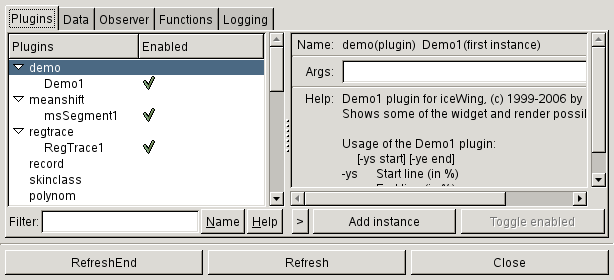
\includegraphics[width=9.4cm]{winPlugPlugins}
    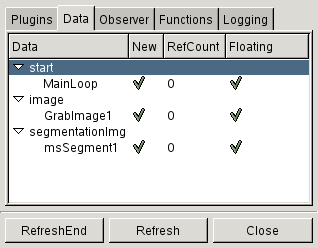
\includegraphics[width=4.7cm]{winPlugData}
    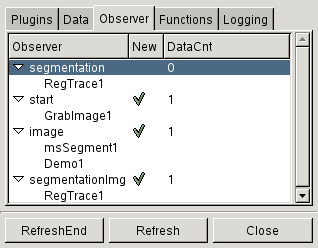
\includegraphics[width=4.7cm]{winPlugObserver}
    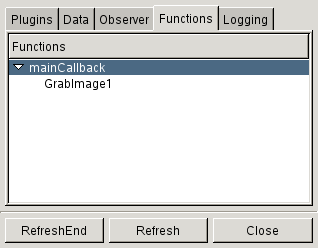
\includegraphics[width=4.7cm]{winPlugFunctions}
    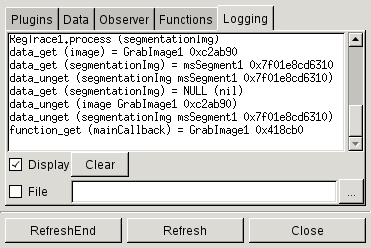
\includegraphics[width=5.45cm]{winPlugLogging}
    \label{fig:windowPlugin}
  \end{center}
  \caption{All pages of the window ``Plugin Info'', which shows
    information about loaded plugins.}
\end{figure}

Inside a main loop \icewing{} calls the registered plugin instances
repeatedly. The order in which the instances get called is defined
by the plugins. For this and for the communication between plugins
\icewing{} offers different functionality. Plugin instances can
provide new data elements, they can observe the provision of data,
and they can call functions of other plugin instances. Details about
these communication possibilities as well as details about all known
plugins is displayed on the different ``Plugin Info'' pages.
The displayed information is not continously updated. By pressing
``Refresh'' the current internal state about the communication
information is displayed immediately. ``RefreshEnd'' defers the
display shortly before the end of the main loop, directly before any
floating data with a reference count of zero gets deleted (see
below). By pressing ``RefreshEnd'' you will get in most of cases
information about all data, which was provided during the last main
loop iteration.

\begin{description}
\item[Plugins] On the first page \emph{``Plugins''} a list of all
  plugins \icewing{} knows about and all instances of these plugins
  is displayed. First all loaded plugins and all its instances are
  shown. The category ``All installed plugins'' is only shown if the
  file ``\$\{PREFIX\}/share/iceWing/\Index{plugins.help}'' is
  available. This file contains information and descriptions about
  the installed plugins. The file is created by the shell script
  ``\verb|icewing-docgen|''\index{icewing-docgen}. See
  section~\ref{sec:icewing-docgen} for more information about this
  script. Pressing the button ``\textgreater{}'' on the lower right
  side of the page displays additional information about the
  currently selected plugin or plugin instance. Displayed are the
  plugin name, for an instance the command line arguments for this
  instance, and the output of the plugin if it is called with the
  command line option ``-h''.

  The filter bar directly below the list allows to limit the
  displayed plugins. Only plugins who's name or who's help string
  contain a certain string are shown in the list. The search is case
  insensitive.

  A double-click on one of the plugin instances (de)activates the
  instance. If an instance is deactivated the process() function of
  this plugin instance is not called anymore. This is similar in
  effect to the command line parameter ``-d''. This function can be
  selected as well in the context menu of the list and via the
  button ``Toggle enabled''. The button ``Add instance'' and the
  corresponding context menu entry create at the start of the next
  main loop run a new instance of the currently selected
  plugin. This is similar to specifying ``-l pluginName'' on the
  command line. The string in the ``Args:'' entry box specifies the
  command line arguments for the new instance.

\item[Data] The \emph{``Data''} page shows information about all data
  the plugins have created. In \icewing{} an identifier, a string, is
  always associated with all data. This identifier allows the plugins
  to access the data. In the first column the identifier and the
  instance name of the plugin, which has made the data available, is
  displayed. All data inside \icewing{} is reference counted and gets
  automatically deleted if the reference count drops to zero. If the
  data is marked as ``floating'' the deletion is deferred until the
  end of one main loop iteration. Data is marked as ``New'' as long
  as one main loop iteration is not finished since the data was
  provided by a plugin instance.

\item[\Index{Observer}] The \emph{``Observer''} page shows
  information about plugin instances, which observe the provision of
  data. If new data with an identifier, which is observed, gets
  provided by any plugins the observer of this data are called with
  the new data as an argument. Thus the order in which instances get
  called is defined by the provision of data and by the observation
  of these data elements. There is one special data element. The
  data ``start'' is not provided by a plugin, but by \icewing{} at
  the start of every main loop run. Plugin instances can observe
  this data and thus get called at the start of the main loop. The
  ``Observer'' page shows the different registered observer and
  information about currently known data elements with a
  corresponding identifier. New data is available, if the data was
  provided during the current main loop iteration. Additionally the
  amount of available data elements with the observed identifier is
  displayed.

\item[Functions] The \emph{``Functions''} page shows information
  about all functions, which plugin instances have published. The
  function identifier and the plugin instance names, which have
  provided the function, are displayed.

\item[\Index{Logging}] The \emph{``Logging''} page allows to get
  more detailed real time information about the communication
  between the plugins. By activating the ``Display'' toggle button
  calls to the different \icewing{} functions, which deal with the
  communication between plugins, are shown in the text widget
  above. For a description of the different functions please see
  section~\ref{sec:p_kommunikation}. The ``Clear'' button clears the
  text widget. Deactivating the toggle button stops the
  logging. Activating the ``File'' toggle button records this
  information in the file, whose name is given in the string widget
  next to the toggle button. The file is closed if the toggle button
  is deactivated.
\end{description}

\subsection{Category ``Images'' and \Index{image windows}}
\label{sub:gui_images}

The category ``Images'' shows a list of all image windows that the
plugins wish to display. Double-clicking an entry of the list
opens or closes the window of that entry.

Every of these image windows \icewing{} or any plugin creates will
have different standard menu entries in a context menu. You can
access this menu by clicking with the right mouse button in an open
image window. Depending on the things a plugin renders in the image,
there might be additional plugin specific entries.

Here is a list of entries you will find in all or, partly, a lot of
image windows:

\paragraph{File/Save}
Saves the actual visible window content, including all active
rendering manipulations. In the preference window of \icewing{} you
can specify different parameters for the saving process, e.g. the
file name and the file format.

\paragraph{File/\Index{Save Original}}
Saves the underlying original ``world coordinate'' image, without
any active rendering manipulations, in the original color space (for
example YUV). But if the downsample factor (page ``other'') is
\textgreater{}1, you will still save downsampled images. This
downsampling happens inside the plugin ``grab'' {\em before} the
original images are anyhow rendered in a image window or passed to
further \icewing{} plugins. Moreover this function does not save any
texts, lines, regions, or anything else besides images the plugin
may display in the image. Only the first image is saved.

\paragraph{File/\Index{Save Seq}}
Once activated, every new acquired image (the visible window
content, including all active rendering manipulations) is saved
continuously until deactivated. Normally, if the active image format
is for single images, a series of image files gets
stored. Otherwise, if one of the AVI file formats is selected, a
single video-stream file is stored. You can change this format in
the preferences window, see section~\ref{sub:preferences} for
further details.

{\em Caution!} If you have selected on of the AVI formats in the
preference window, you must remember: To prevent corrupt AVI files,
you must end this ``Save Seq'' by (de)selecting this command in the
context menu again and continue with at least one new image to close
the saved AVI file. Alternatively while recording you can close the
whole image window or end \icewing{} with the ``Quit'' button, and
\icewing{} sends the close file command itself. Changing the Image
format in the preference window will do the same. If the file is not
closed the AVI will miss some finalizing code and thus will be
corrupt.

\paragraph{File/Save OrigSeq}
Same as ``Save Seq'', but the original ``world coordinate'' images
are used. For the data, which gets saved by this function the same
as already stated under ``Save Original'' applies.

\paragraph{File/Save Session}\index{session file}
Saves the current \icewing{} window configuration under the
currently active session name. On the next start of \icewing{} every
currently open window will be remembered as it is. Without any
special parameters the next time \icewing{} is launched, the default
configuration-file in ``\$\{HOME\}/\Index{.icewing/session}'' will
be used to restore any windows. Alternatively, the command line
parameter ``-ses \textless{}session-file\textgreater{}'' can be used
to switch to non-default session files.

The Save/Clear Session menu entries are the same commands as the
ones in the preferences-window.

\paragraph{File/Clear Session}
This physically deletes the current session file and thus clears the
session. At the next launch the window layout of \icewing{} will
look like the inbuilt default.

\paragraph{File/Close Window}
Closes the window.

\paragraph{View}\index{Pan window}\index{Zoom window}
The View submenu contains different entries to zoom and pan inside
the image windows. So these entries are alternatives to the middle
mouse button and the scroll whell. See section~\ref{sub:panZoom} for
more details. The menu is especially handy if the entries are called
via hotkeys. Besides using predefined hotkeys, the hotkeys of all
menu entries can be dynamically changed. If a menu entry has
currently the focus of the mouse a new hotkey can be set by simply
pressing the desired hotkey. All hotkeys are saved in the
configuration file.

\paragraph{\Index{Info Window}}
Opens a small window, which displays the coordinates and color in
several color spaces of the pixel at the mouse position if the
mouse is inside any image window. Additionally, if the mouse is over
any rendered images, the ``Original'' tab shows information about
the data at the mouse position as it was passed to the \icewing{}
render functions. For example \icewing{} can display images
containing float values, which are converted to 8 bit integer values
during display. Possibly, these values are further changed by any
special rendering filters or any drawings, which are shown above the
image. These final 8 bit values are then displayed as the color
values. In contrast, the ``Original'' tab shows the float values
from the inital image.

The spin button allows to set the radius of the square area, from
which the displayed color values are averaged. A radius of ``0''
uses only the pixel under the mouse cursor. The ``Original'' tab
considers the zooming value. The ``Display'' tab ignores the zoom
value.

Additionally, this window contains two toggle buttons for two
special functions. If the ``\Index{color picker}'' is pressed, the
info window waits on a press with the left mouse button inside one
of the image windows. The values at the time the button was pressed
are then additionally displayed in the info window. Thus two
positions can be easily compared. \index{measure distances}If
``measure'' is pressed, distances and angles in the image windows
can be measured. If the left mouse button is pressed inside an image
window and then moved to a second position, the distance of these
two positions and the angle between a horizontal line and the marked
line are displayed in the info window. Afterwards, to change the
initially selected line, the end points of the marked line can be
dragged around.

\paragraph{Remember Data}
(De-)activates the ``Remember Data'' mode, that was already
discussed in detail in section~\ref{sec:renderchain}.

\paragraph{Settings}
Opens a window, where you can change some further image window
related options. As one point different options for the ``Show
\Index{Meta info}'' feature and the image rendering can be
specified. Moreover, all plugins can add any widgets to this
window. For a description of these options please refer to the
special plugin documentation.\\ The meta info / image rendering
related options are:
\begin{quote}
\begin{description}
\item[\Index{Histogram}] ``Show Meta info'' displays histograms of
  all rendered images. Here you can influence these histograms.
  ``Use lines'' changes the visualization form of the histograms
  (filled or single lines). ``Include min/max'' changes the method
  used for scaling the histogram in the vertical axis. If activated,
  the biggest value of the histogram is used to scale the
  histogram. If deactivated, the first and the last histogram
  entries are not considered during determining the biggest value of
  the histogram. Useful, if a small object is located on an
  otherwise black or white image.
\item[Planes which should be shown] Images can have any number of
  planes. Normally, plane 0 of input images is shown in image
  windows for gray images and the planes 0, 1, and 2 are shown in
  color based image windows. With this text entry the used planes
  can be changed. For example, by entering ``4 0 1'' plane 4 of the
  input image is used as the first displayed plane (the ``red''
  plane for an RGB image), plane 0 as the second (``green'' plane),
  and plane 1 for the third one (``blue'' plane). By entering ``2'',
  only the plane 2 is shown even in color based image windows.
\item[\Index{scaleMin/Max}] Images in \icewing{} can have any data
  type ranging from unsigned chars to doubles. For displaying these
  images must be converted to a range of 0 to 255. With these
  sliders you can influence the conversion process. With ``scaleMin
  = -2'' the image values are simply shifted in the range 0..255
  without locking further at the image values, e.g. for unsigned
  short images 65535 is displayed with a value of 255. ``scaleMin
  = -1'' clamps the image values to a range of 0..255.

  All other values for the sliders consider the minimal and maximal
  values of the to be displayed image. The Min slider specifies the
  amount, the minimal value is shifted towards the maximal value, in
  percent of the difference of the minimal value and the maximal
  value. The Max slider shifts the maximal value towards the minimal
  value. All pixels darker then the shifted minimal value are
  displayed as black, all pixels lighter then the maximum are
  displayed as white, and everything in between is stretched
  linearly.
\end{description}
\end{quote}

\paragraph{Entries of the submenu Preview}

\begin{description}
\item[Normal] Shows the image in the window with the original colors
  as they were specified during rendering.

\item[CStretch] \index{Contrast autostretch}The color histogram of
  the image is stretched: The minimum (and maximum) of all used
  colors is set to 0 (255) and all colors are stretched linearly to
  the full range 0~-~255 again.

\item[CStretch5] 5\%, beginning with the nearest to black (white)
  pixels are set to black (white). All other colors are stretched
  linearly.

\item[CStretch10] Same as CStretch5, but with 10\% of all pixels to
  black/white.

\item[HistEQ] \index{Histogram equalize}
  Equalize the histogram of the image.

  Equalization is used to repair images that have too much contrast
  or are too light or dark. Equalization attempts to flatten the
  histogram of the image.

\item[Random] This randomly shuffles the color map.

  Colors of the original image, that look very similar, change to
  very distinguishable colors. This is very useful to e.g. verify
  some color-separation processes.
\end{description}

\paragraph{Show MetaInfo}\index{Meta info}
This menu entry appears only if images are displayed in the window.
``Show MetaInfo'' (de-)activates the display of some additional
information of the original image as passed to the render functions,
for example the color-space of the input image, the size of the
image in pixels and the color histogram of the image.

\paragraph{Font}
This menu entry appears only if text may be displayed in the window.
Selects the font and thus the size of any text, which get rendered
inside the image window (for example the text shown if the meta info
is activated).

\paragraph{\Index{Font Shadows}}
This menu entry appears only if text may be displayed in the window.
Shows the rendered text with shadowed fonts. Helps sometimes to make
the text more visible.

\subsection{Panning/Zooming the image windows}
\label{sub:panZoom}
\index{Pan window|idxmain}
\index{Zoom window|idxmain}

If a new image window is opened the rendered image is normally
displayed in such a zoom level that it is always completely
visible. By pressing the shift key and the middle mouse button
inside the window you can zoom into the image, by pressing the ctrl
key and the middle mouse button you can zoom out. Alt plus the
middle mouse button resets to the initial fit to window displaying
mode. If fit to window is \emph{not} active you can hold the middle
mouse button and move around inside the window to move the clipping
frame for the ``world coordinate'' picture, i.e. to pan inside the
image.

\emph{Attention:}\\
If your window manager is already using one or more of that
combinations for itself, then that signal can not reach \icewing{}!
If you want to use the function, you have to change your window
manager setting: Disable that mouse signal there, so it will no
longer get caught by your window manager and can reach \icewing{}.

Besides using the middle mouse button for zooming and panning, there
are two additional posibilities to reach these functions: by using
the \Index{mouse wheel} or the context menu. For panning the window
vertical, again if fit to window is \emph{not} active, you can use
the mouse wheel. Panning horizontally can be done with the mouse
wheel while pressing the shift key and zooming by using the mouse
whell while the ctrl key is pressed. Additionally, the image context
menu contains a submenu ``View'' with entries for all these
functions.


%######################
\section{The GUI widgets}

(TODO: FULL list, or only short summary?)
Widget ``List'' can have a context menu. And it can be reordered via
drag'n drop...

In Goptions.h
opts\_xxx\_create()

\chapter{Plugins of the default distribution}

The \icewing{} package already contains different plugins. This
chapter gives a brief overview over all these plugins. Some of the
plugins are directly compiled into \icewing{} and some others are
normal external plugins. The external plugins are not installed
during the normal \icewing{} installation. They have to be compiled
and installed separately. See the quicktour,
section~\ref{sec:quicktour}, for an example of how to install a
plugin.

\section{Plugin grab}
\index{Plugin!grab}\index{grab plugin}

The plugin grab is an inbuilt plugin, that allows to acquire images
or video streams from grabber hardware, disk or via \dacs{} from
external processes. The plugin provides the images under the
identifier ``image'' (YUV color space) and optionally under the
identifier ``imageRGB'' (RGB color space) under the data type
``grabImageData'', see page~\pagereftop{page:p_grabImageData}. As
grab is an often used and very central plugin it was already
described in detail in the manual. Especially
sections~\ref{sec:commandline} and \ref{sub:gui_grab} covered the
grab plugins command line interface and its user interface.

\section{Plugin demo}
\index{Plugin!demo}\index{demo plugin}

An external plugin demonstrating all widgets available in \icewing{}
and the different render capabilities of \icewing{}. The quicktour,
section~\ref{sec:quicktour}, used this plugin for a first \icewing{}
demonstration.

\section{Plugin min}
\index{Plugin!min}\index{min plugin}

An external plugin showing the basic structure of an \icewing{}
plugin. The plugin does not do anything usefull, it shows only the
structure of a complete plugin. This plugin is used in the
section~\ref{sec:p_overview} to introduce plugin programming. If you
want to create own plugins be aware that there is also a plugin
generator, icewing-plugingen, which is documented in
section~\ref{sec:icewing-plugingen}. This tool generates a nicer
starting point for own plugins.

\section{Plugin min\_cxx}
\index{Plugin!min\_cxx}\index{min\_cxx plugin}

An external plugin showing the basic structure of an \icewing{}
plugin. It's nearly identical to the min plugin besides that it uses
the C++ plugin interface of \icewing{}. Similar to the min plugin
this plugin is used in the section~\ref{sec:p_overview} to introduce
plugin programming. If you want to create own plugins be aware that
there is also a plugin generator, icewing-plugingen, which is
documented in section~\ref{sec:icewing-plugingen}. This tool
generates a nicer starting point for own plugins.

\section{Plugin record}
\index{Plugin!record}\index{record plugin}

The record plugin is compiled into \icewing{} and performs optimized
saving of images by using a second thread to write the images to disk.
Additionally it has support to drop single frames in a controlled
manner. If started without arguments the plugin gets called for data
with the identifier ``image'' of type ``grabImageData'', the
identifier the grabbing plugin uses to provide its images for other
plugins. The observed data can be changed via its command line
interface.

\subsection{Command line parameter}

\begin{description}
\item[-g \textless{}ident\textgreater{}]
  Observe data of type ``grabImageData'', the default (with ident =
  ``image'') if neither ``-g'' nor ``-i'' is specified. Besides the
  image data this data type additionally contains grabbing time and
  file name information, which can be used to name the saved files.
\item[-i \textless{}ident\textgreater{}]
  Observe data of type ``iwImage''. This format contains only image
  information.
\end{description}

\subsection{User interface}

\begin{description}
\item[Plugins to handle] Normally, the plugin is called successively
  for all images which are stored under one ident. E.g. if two
  grabbing plugins were started in parallel, the plugin is called
  two times for both of these images. Here you can restrict the
  calling of the plugin to data elements from only a subset of
  the plugins. E.g. if you want to save only images from the second
  grabbing plugin, you can select the second grabbing plugin with
  this widget.
\item[Record]\hfill
  \begin{description}
  \item[Off:] The plugin does nothing.
  \item [Exclusive:] The received images are saved and the processing
    of any further plugins during the current main loop run is
    canceled. Beware: If the record plugin should handle more than
    one image (for example the two images from two parallel started
    grabbing plugins), this toggle can \emph{not} be set to
    ``Exclusive'', otherwise the plugin would not be called for the
    second image nor for any further ones.
  \item[Parallel:] The received images are saved to disk without
    disturbing any other plugin processing.
  \item[Once:] The plugin processes the images until it is called a
    second time for an image from a plugin which was already
    processed. After that processing is deactivated automatically.
  \end{description}
\item[Framedrop] The plugin maintains a queue where all received
  images are added. A second thread continously removes images from
  this queue and saves them to disk. If this slider is not 0, the
  main thread can wait some ms if the queue gets to long so that the
  second thread has more time to save the images. If the queue is
  longer than 4 times the slider value, the main thread waits 200ms,
  if it's longer than 2 times, the thread waits 80ms, and if the
  queue is longer than 1 times the slider value the thread waits
  40ms.
\item[Convert to RGB] If selected, the received image data is
  converted from the color space YUV to to the color space RGB
  before saving. This is ignored for all movie formats.
\item[Image format] Specifies the file format used for saving
  images. If ``By Extension'' is selected, the format gets selected
  based on the extension of the file name. The different image
  formats are described in more detail on
  page~\pagereftop{page:gui_image_format}.
\item[Framerate based dup/drop-frames] If AVI files of the formats
  AVI YUV444, AVI YUV420, or AVI MJPEG are saved and this toggle is
  active, frames get duplicated or dropped to adapt to the selected
  frame rate.
\item[AVI Framerate] If AVI files get saved, this value determines
  the desired frame rate. Frames are duplicated or dropped to adapt
  to this value if the toggle button above this slider is
  active and the selected file format is AVI YUV444, AVI YUV420, or
  AVI MJPEG. Otherwise this value is only stored in the header of
  the saved AVI file.
\item[Quality] The quality and thus the compression value used when
  saving jpeg images or AVI movies encoded as MJPEG or MPEG-4. 100
  means a small compression and thus a good quality. For MPEG-4
  files this sets the desired bits per pixel from 0.05 to 0.5.
\item[File Name] The file name, under which the images will be
  saved. You can embed different information in the name by using
  the following modifiers:
  \begin{tabbing}
    \%T\=: \= \kill
    \%d\>:\> The consecutive image saving counter, starting at 0.\\
    \%t\>:\> The milliseconds part of the time the image was grabbed/loaded.\\
    \%T\>:\> The seconds part of the time the image was grabbed/loaded.\\
    \%b\>:\> The name of the current user\index{user name}.\\
    \%h\>:\> The system's \Index{host name}.\\
    \%p\>:\> The images file path part of its complete file name.\\
    \%f\>:\> The images file name part of its complete file name.\\
    \%e\>:\> The images file extension part of its complete file name.\\
    \%F\>:\> If the input was a video, the number of the current frame, otherwise 0.\\
    \%P\>:\> The name of the plugin which provided the current image.
  \end{tabbing}
  Any of the above modifiers can be changed by printf() style format
  specifiers. E.g. ``image\%03d.ppm'' would result in
  ``image000.ppm'', ``image001.ppm'' and so on as file names.
\item[Reset \Index{FilenameCounter}] By using \%d in the file name, a
  consecutive image saving counter is embedded in the image file
  name. This button resets this value to zero. If currently image
  recording is active the resetting is done after the recording is
  again switched off.
\end{description}

\section{Plugin remotectrl}
\index{Plugin!remotectrl}\index{remotectrl plugin}
\label{sec:remotectrl}

\index{Internet socket}
An external plugin which allows to remote control \icewing{} with an
own Internet sockets based communication protocol and optionally the
\Index{XCF framework}. See \url{http://xcf.sourceforge.net} for more details
about the external XCF framework. The plugin uses the capability of
\icewing{} to save and load all its current status into a
configuration file. Remote control works quite similar: The plugin
publishes the functions ``void control(char[])'' and ``char[]
getSettings(void)''. The ``char[]'' means, that you send a normal
C-string as parameter to the ``control()'' function. The content of
that string can be any lines of the \icewing{} configuration file
and \icewing{} accepts the new settings. Similar, the
``getSettings()'' function returns a string with the current
settings of all widgets in the format of the configuration file.

The plugin works similar to the \icewing{} ``-of'' option from
page~\pagereftop{page:opt_of} for remote controlling via \dacs{}.
See also the icewing-control program from the utils directory for a
utility, that allows to send such strings to a running \icewing{}
instance. The utility supports the internal sockets based
communication protocol, the XCF framework, as well as the \dacs{}
framework. See section~\ref{sec:icewing-control} for more details
about this utility.

\subsection{Command line parameter}

\begin{description}
\item[-p [port{]}]
  Use the own internal Internet sockets based communication protocol
  to provide the two functions. The parameter gives the port of the
  socket, the default is 4208. If port 0 is given, a free port is
  selected automatically and printed to stderr.

  This is the default if neither ``-p'' nor ``-x'' is given.
\item[-x [name{]}]
  Use the XCF framework to provide the two functions. The parameter
  gives the name of the XCF server the plugin uses for publishing
  the two functions. The default is ``xcf''.
\end{description}

\section{Plugin shmdata}
\index{Plugin!shmdata}\index{shmdata plugin}
\index{Unix domain socket}

An external plugin which allows to distribute data via \Index{shared
 memory} and local unix domain sockets to any number of other local
processes, i.e it allows unidirectional one to n
communication. Supported are data elements of type
``grabImageData'', ``iwImage'', and char[].

An example invocation to distribute the images from a grabbing
plugin on the sender side and provide them on the receiver side
under the same identifier would be:\\
\begin{small}
\shellcom{icewing -sp SomeImages -l shmdata -a shmData1 ``-p test -g image''}
\end{small}
on the sender side and\\
\begin{small}
\shellcom{icewing -l shmdata -a shmData1 ``-p test -o image''}
\end{small}
on the receiver side. The command from the receiver side can be
invoked multiple times to distribute the image to multiple
\icewing{} processes.

\subsection{Command line parameter}

\begin{description}
\item[-p \textless{}socket\textgreater{}]
  The name of the socket for the communication channel. It will be
  prefixed with ``/tmp/''. This parameter must be given always on
  the sender as well as on the receiver side.
\item[-g \textless{}ident\textgreater{}]
  Observe data of type ``grabImageData''. For example the grabbing
  plugin provides this data type under the idents ``image'' and
  ``imageRGB''. Exactly one of ``-g'', ``-i'', and ``-s'' must be
  given on the sender side.
\item[-i \textless{}ident\textgreater{}]
  Observe data of type ``iwImage''. Exactly one of ``-g'', ``-i'',
  and ``-s'' must be given on the sender side.
\item[-s \textless{}ident\textgreater{}]
  Observe data of type char[]. Exactly one of ``-g'', ``-i'', and
  ``-s'' must be given on the sender side.
\item[-n \textless{}num\textgreater{}]
  The sender copies the to be send data to a new shared memory
  region and informs all receivers about it. The receivers inform
  the sender when they do not need the data any more so that the
  sender can free the memory region. This number specifies the
  maximum number of items the sender allocats at the same time
  before the sender waits that the receivers notify him for memory
  not needed any more. The default is 2.
\item[-o \textless{}ident\textgreater{}]
  The identifier under which the receiver provides the received
  data. Must be given exactly one time on the receiver side.
\item[-b]
  Normally the receiver blocks until new data from the sender is
  available. If ``-b'' is specified, the receiver plugin does not
  block but simply finishes without storing any new data.
\end{description}

\subsection{User interface}

\begin{description}
\item[\Index{Wait Time} and Receive Next]
  The slider sets the delay (in milliseconds) until the next image
  shall be acquired from the sender side. If you set it to -1,
  \icewing{} waits until you manually press the ``Receive Next''
  button. This -1 works like a ``pause-mode''.
\end{description}

\section{Remaining plugins}

The following plugins belong all to a project about hand
segmentation and tracking. They are all (a) compiled into
\icewing{}, (b) somewhat old, and (c) probably not really generally
useful.

\begin{description}
\item[imgclass]\index{Plugin!imgclass}\index{imgclass plugin}
  Performs color classification of the input image by using a lookup
  table.
\item[skinclass]\index{Plugin!skinclass}\index{skinclass plugin}
  Segment skin colored regions. Needs at least one other plugin to
  perform the real color classification.
\item[backpro]\index{Plugin!backpro}\index{backpro plugin}
  Perform color classification based on back projection. Needs the
  skinclass plugin.
\item[gsimple]\index{Plugin!gsimple}\index{gsimple plugin}
  Perform color classification with a gauss distribution. Needs the
  skinclass plugin.
\item[polynom]\index{Plugin!polynom}\index{polynom plugin}
  Perform color classification with a lookup table. This plugin
  needs the skinclass plugin.
\item[tracking]\index{Plugin!tracking}\index{tracking plugin}
  Track regions with a kalman filter. Needs the skinclass plugin.
\end{description}

\chapter{Programs of the default distribution}

Besides the main \icewing{} program the \icewing{} package contains
some additional tools and utilities. This chapter gives a brief
overview over all these tools. Most of the tools are installed
during the normal installation as described in
chapter~\ref{chap:installation}. One tool, the icewing-control
program, is only build and installed during the main install process
if the CMake build system is used. Otherwise it has to be installed
separately.

\section{icewing}
\index{iceWing!icewing program|idxmain}

The icewing program is the main program of the \icewing{}
package. This program was already described in detail in this
documentation.

\section{icewing-config}
\index{icewing-config|idxmain}\label{sec:icewing-config}

icewing-config is a shell script similar to e.g. gtk-config which
makes compiling of own plugins easy. It generates compiler-flags,
extracts system-paths, and more. ``\verb|icewing-config --help|''
shows all available options of the script. In detail these are

\begin{description}
\item[--prefix] Prints the installation directory of the \icewing{}
  package to stdout.
\item[--bindir] Prints the directory \$\{PREFIX\}/bin, i.e the
  directory ``bin'' under the installation directory, to stdout.
\item[--libs] Print the linker flags that are necessary to link an
  \icewing{} plugin to stdout. I.e. the output of this command
  should be used during linking of own plugins.
\item[--cflags] Print the compiler flags that are necessary to
  compile an \icewing{} plugin to stdout. I.e. the output of this
  command should be used during compiling of own plugins.
\item[--libdir] Prints the directory \$\{PREFIX\}/lib/iceWing, i.e the
  directory ``lib/iceWing'' under the installation directory, to
  stdout. This is the directory where new plugins should be
  installed.
\item[--datadir] Prints the directory \$\{PREFIX\}/share/iceWing, i.e
  the directory ``share/iceWing'' under the installation directory,
  to stdout. This is the directory where plugins can store any
  data files. Additionally, \icewing{} itself stores some data files
  in this directory.
\item[--pincludedir] Prints the directory
  \$\{PREFIX\}/include/iwPlugins, i.e the directory
  ``include/iwPlugins'' under the installation directory, to
  stdout. This is the place where plugins can install new header
  files.
\item[--home=HOME] If specified, use HOME instead of
  \urltilde{}/.icewing for the --libdir-home, --datadir-home, and
  --pincludedir-home options. This option must come before these
  three ``-home'' options to take effect. This option can be used to
  adapt the ``-home'' options to the \Index{ICEWING\_PLUGIN\_PATH}
  environment variable.
\item[--libdir-home] Prints the directory
  \urltilde{}/.icewing/plugins to stdout. This is an alternative
  directory to the one from --libdir where new plugins can be
  installed.
\item[--datadir-home] Prints the directory \urltilde{}/.icewing/data
  to stdout. This is an alternative directory to the one from
  --datadir where plugins can store any data files.
\item[--pincludedir-home] Prints the directory
  \urltilde{}/.icewing/include to stdout. This is an alternative
  directory to the one from --pincludedir where plugins can install
  new header files.
\item[--version] Prints the version number of \icewing{} to stdout.
\end{description}

As an alternative to icewing-config a metadata file for
\Index{pkg-config} is installed as well. E.g. ``pkg-config --cflags
icewing'' will print the necessary compiler flags for compiling an
\icewing{} plugin. All the other information icewing-config provides
can be as well retrieved with pkg-config. The only difference is
that pkg-config does not support variable names with ``-'' in its
names, so ``\_'' is used instead.

\section{\Index{icewing-control}}
\label{sec:icewing-control}

icewing-control allows to remote control \icewing{}. The tool uses
the capability of \icewing{} to save and load all its current status
into a configuration file. Remote control works quite similar: The
tool can send a string containing any lines of the \icewing{}
configuration file to a running \icewing{} instance and can receive
a string from \icewing{} containing the complete current
configuration.

\index{XCF framework}\index{Internet socket}\index{DACS}
\icewing{} has to be started with the ``-of'' option or the
remotectrl plugin has to be used. If the option ``-of'' is used,
\dacs{} communication is used and icewing-control must be started
with the ``-n'' option. If the remotectrl plugin is used, native
sockets based communication or XCF based communication can be used
and icewing-control must be started with the corresponding ``-p'' or
``-x'' option to allow communication between \icewing{} and the
icewing-control tool. See page~\pagereftop{page:opt_of} and
section~\ref{sec:remotectrl} for more details about the ``-of''
option and the remotectrl plugin.

``\verb|icewing-control --help|'' shows all available options of the
tool. In detail these are
\begin{description}
\item[-p [host:port{]}] Use the own internal Internet sockets based
  protocol for communication with the remotectrl plugin of a running
  \icewing{} instance. The argument gives the location where the
  remotectrl plugin is running. The default is
  \mbox{``localhost:4208''}.
\item[-n [name{]}] Use \dacs{} for communication with a running
  \icewing{} instance. The argument is the \dacs{} name of the
  icewing program as specified with the \icewing{} ``-n'' option
  (see page~\pagereftop{page:opt_n_name}). The default is
  ``icewing''.
\item[-x [xcf-server{]}] Use XCF for communication with the remotectrl
  plugin of a running \icewing{} instance. The argument is the XCF
  server name of the remotectrl plugin as specified with the
  remotectrl ``-x'' option (see section~\ref{sec:remotectrl}). The
  default is ``xcf''.
\item[-g] Call the ``char[] getSettings(void)'' function to get all
  current widget settings and print them to stdout. Exit
  icewing-control after all command line options have been
  processed.
\item[-s config-setting] Call the ``void control(char[])'' function
  to set the specified widgets to the specified values and exit
  icewing-control after all command line options have been
  processed. An example would be
  ``\verb|-s "GrabImage1.Wait Time = 94"|'' to set the ``Wait Time''
  button on the ``GrabImage1'' page to 94.
\end{description}

If neither any ``-g'' nor any ``-s'' option is given, an interactive
shell is started. The shell supports TAB completion for commands and
its arguments. The available commands are
\begin{description}
\item[help] Show all available commands.
\item[get] Get all iceWing settings and print them to stdout. This
  is identical to the ``-g'' option.
\item[set] Set one widget in iceWing to a new value. For example the
  command ``\verb|set GrabImage1.Wait Time = 94|'' sets the
  ``Wait Time'' button on the ``GrabImage1'' page to 94. This is
  identical to the ``-s'' option.
\item[quit] Quit the icewing-control tool.
\end{description}

\section{icewing-docgen}
\index{icewing-docgen|idxmain}\label{sec:icewing-docgen}

icewing-docgen is a shell script which collects help messages of all
plugins which are installed under \$\{PREFIX\}/lib/iceWing and all
plugins which are integrated in \icewing{}. The script calls all
these plugins with the option ``-h'' and stores the output in the
files ``Readme.txt'' and ``Readme.html'' in the current
directory. Additionally, it copies the file ``Readme.txt'' to
``\$\{PREFIX\}/share/iceWing/\Index{plugins.help}''. This file is
used by \icewing{} to display additional information about plugins
on the ``Plugins'' page in the ``Plugin Info'' window. See
section~\ref{sub:PluginInfo} for information about this window. You
should use this script every time after installing new plugins.

\section{icewing-plugingen}
\index{icewing-plugingen|idxmain}\label{sec:icewing-plugingen}

icewing-plugingen is a \Index{plugin template generator}. The script
generates in the current directory a basic C or C++ plugin including
a Makefile to compile it. The plugin is directly compiled for
immediate testing. The plugin is kept short and simple, but shows
already data observation, easy user interface generation, and
rendering of data in a window.

``\verb|icewing-plugingen --help|'' gives more information about its
invocation. It is a shell script which expects up to three
arguments:
\sS
\shellcom{icewing-plugingen [-c|-cxx|-cpp] plugin-name short-name}
\begin{description}
\item[-c] If given, a new C-plugin of name ``plugin-name'' is
  generated in the current directory. Function and type names in the
  generated source start with ``short-name''. This option is the
  default if none of the three is given.
\item[-cxx] If given, a new C++-Plugin of name ``plugin-name''
  deriving from the class Plugin is created in the current
  directory. 
\item[-cpp] This is a synonym for -cxx. See there for a description
  of the option.
\end{description}

%%% Local Variables: 
%%% mode: latex
%%% TeX-master: "../iceWing"
%%% fill-column: 68
%%% End: 
